% Dokumentklassen sættes til memoir.
% Manual: http://ctan.org/tex-archive/macros/latex/contrib/memoir/memman.pdf
\documentclass[a4paper,oneside]{article}

% Ingen nummering af overskrifter
\setcounter{secnumdepth}{0}

% Danske udtryk (fx figur og tabel) samt dansk orddeling og fonte med
% danske tegn. Hvis LaTeX brokker sig over æ, ø og å skal du udskifte
% "utf8" med "latin1" eller "applemac".
\usepackage[utf8]{inputenc}
\usepackage[danish]{babel}
\usepackage[T1]{fontenc}

\usepackage{float}

% Matematisk udtryk, fede symboler, theoremer og fancy ting (fx kædebrøker)
\usepackage{amsmath,amssymb}
\usepackage{bm}
\usepackage{amsthm}

% Kodelisting. Husk at læse manualen hvis du vil lave fancy ting.
% Manual: http://mirror.ctan.org/macros/latex/contrib/listings/listings.pdf
\usepackage{pxfonts}
\usepackage{listings}
\lstset{language=VHDL,
	basicstyle=\ttfamily,
	keywordstyle=\bfseries,
	frame=single,
	numbers=left,
	breaklines=true,
	numberstyle=\footnotesize,
	tabsize=4, 
	showstringspaces=false
	%morekeywords={include, printf}
}

% Fancy ting med enheder og datatabeller. Læs manualen til pakken
% Manual: http://www.ctan.org/tex-archive/macros/latex/contrib/siunitx/siunitx.pdf
\usepackage{booktabs}

% Indsættelse af grafik.
\usepackage{graphicx,wrapfig}
%\usepackage[section,subsection,subsubsection]{extraplaceins}
\begin{document}

	
\newcommand{\HRule}{\rule{\linewidth}{0.1mm}} % Defines a new command for the horizontal lines, change thickness here
	
\begin{center}
	
\textsc{\LARGE Ingeniørhøjskolen Aarhus}\\[1.5cm] %

\textsc{\large Digital system design}\\[2.5cm] 
\HRule \\[0.8cm]
{\huge \bfseries \textsc{Journal 1}}\\[0.4cm]
\HRule \\[1.5cm]

\textsc{\large Hold 50}\\
\vspace{0.5 in}
\begin{tabular}{c c c}
	Cecilie Moriat &  Alexander Bennedsen & Lasse Stenhøj \\
	\textsl{201405949} & \textsl{201310498} & \textsl{201407500}
\end{tabular}

\vspace{2.5 in}

{\large\textit{\today}} \\[3cm]
\vfill % Fill the rest of the page with whitespace
\end{center} % Center everything on the page


\renewcommand{\lstlistingname}{Kode}

\tableofcontents

\newpage
\section{Øvelse 2}
\subsection{Opgave 1 - Half-adder}
\begin{enumerate}
	\item[1)]
	Architecture body i VHDL kan skrives på tre forskellige måder; dataflow, behavioral og structural. \\
	Half-adder beskrives i Dataflow style ved hjælp af direkte implementering af logiske gates. Skrivemåden gør det nemt at overføre programmet direkte til hardware og de logiske gates. \\
	I Behavioral style opskrives half-adderen ved brug af if/else statements. Dette giver en god forståelse af selve half-adderens funktion, men det er kompliceret at overføre det til logiske gates ud fra kodens syntax. \\
	I structural style laves et miks af de to ovenstående, da der først defineres en funktion for hver logisk gate som det ses i dataflow style, og derefter implementeres funktionerne i halfadder entity’en. Denne style er god at bruge, hvis man skal implementere en funktion flere gange.\\
	\item[2)]
	Et RTL view af de tre forskellige måder at skrive en half-adder på, giver følgende forskellige resultater:\\
\begin{figure}[h]
	\centering
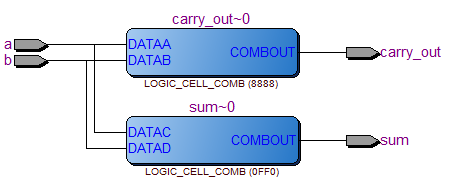
\includegraphics[scale=0.8]{pictures/Oevelse1/Half_adder/Behavioral.JPG}
\caption{Half-adder - Behavioral RTL view}
\label{fig:HaBehavioralRTL}
\end{figure}

\begin{figure}[h]
	\centering
	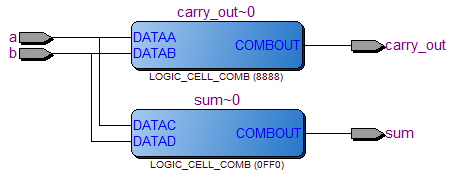
\includegraphics[scale=0.8]{pictures/Oevelse1/Half_adder/dataflow.JPG}
	\caption{Half-adder - Dataflow RTL view}
	\label{fig:HaDataflowRTL}
\end{figure}

\begin{figure}[h]
	\centering
	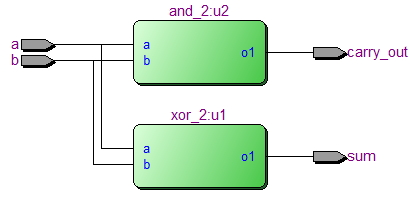
\includegraphics[scale=0.8]{pictures/Oevelse1/Half_adder/Structural.JPG}
	\caption{Half-adder - Structural RTL view}
	\label{fig:HaStructuralRTL}
\end{figure}
	\newpage
	
	Ud fra ovenstående figurer ses det, at dataflow-style og behavioral-style "afkodes" på samme vis, hvor de blå bokse symboliserer en logisk funktion. I structural-style angiver de grønne bokse, også logiske funktioner, men disse er defineret af os, som hhv en AND-funktion og en XOR-funktion. Det er altså med structural-style at vi nemmest kan se, hvilke gates vi skal bruge i en fysisk opbygning af systemet.\\

	\item[3)]
	Følgende tre figurer viser en Timing simulation af hver style. \\
\begin{figure}[h]
	\centering
	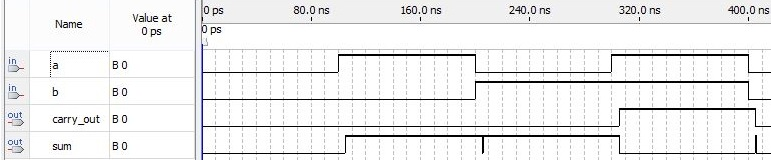
\includegraphics[scale=0.6]{pictures/Oevelse1/Half_adder/Behavioral_timing_simulation.jpg}
	\caption{Half-adder - Behavioral Timing Simulation}
	\label{fig:HaBehavioralTimingSim}
\end{figure}
\begin{figure}[h]
	\centering
	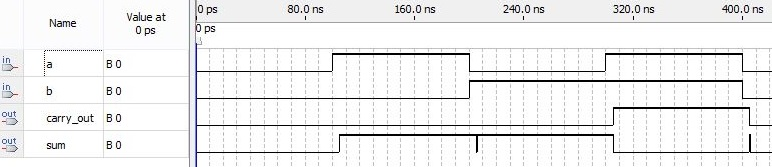
\includegraphics[scale=0.6]{pictures/Oevelse1/Half_adder/Dataflow_timing_simulation.jpg}
	\caption{Half-adder - Dataflow Timing Simulation}
	\label{fig:HaDatalfowTimingSim}
\end{figure}
\begin{figure}[h]
	\centering
	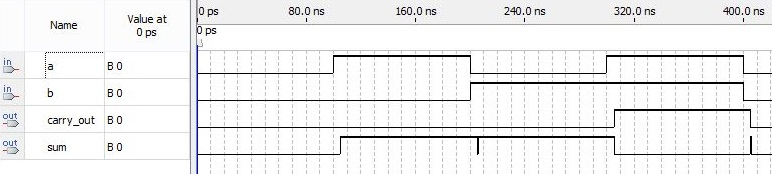
\includegraphics[scale=0.6]{pictures/Oevelse1/Half_adder/Structural_timing_simulation.jpg}
	\caption{Half-adder - Structural Timing Simulation}
	\label{fig:HaStructuralTimingSim}
\end{figure}
	\newpage
	Som det ses på figurerne, forekommer der nogle spikes på funktionerne. Dette skyldes static hazard, da de "gates" vi bruger i vores half-adder, vil have en lille tidsforskydning fra hinanden, og dermed kan give forkerte resultater i brøkdelen af et nanosekund, som det eksempelvis ses når både a-signalet og b-signalet ændrer status.
	\item[4)] 
	For at undgå disse spikes laver vi en functional simulation. Denne slags simulering tager højde for static hazard, og optimerer diagrammet til at vise et "perfekt" resultat.\\
	Figur \ref{fig:HaDataflowFunctionalSim}, \ref{fig:HaBehavioralFunctionalSim} og \ref{fig:HaStructuralFunctionalSim} viser denne type simulering.\\
\begin{figure}[h]
	\includegraphics[scale=0.6]{pictures/Oevelse1/Half_adder/Dataflow_functional_simulation.jpg}
	\caption{Half-adder - Dataflow functional Simulation}
	\label{fig:HaDataflowFunctionalSim}
\end{figure}
\begin{figure}[h]
	\includegraphics[scale=0.6]{pictures/Oevelse1/Half_adder/Behavioral_functional_simulation.jpg}
	\caption{Half-adder - Behavioral functional Simulation}
	\label{fig:HaBehavioralFunctionalSim}
\end{figure}
\begin{figure}[h]
	\includegraphics[scale=0.6]{pictures/Oevelse1/Half_adder/Structural_functional_simulation.jpg}
	\caption{Half-adder - Structural functional Simulation}
	\label{fig:HaStructuralFunctionalSim}
\end{figure}
	\newpage
\end{enumerate}

\subsection{Opgave 2 - Full-adder}
	\flushleft
\begin{enumerate}
	\item[1)]
	Med to half-addere kan man lave en full-adder. Dette vil vi nu implementere i hhv. dataflow-style, behavioral-style og structural-style.\\
	\medskip
	\begin{lstlisting}[caption={Full-adder Dataflow VHDL kode},label={lst:FaDataflowCode}]
	library ieee;
	use ieee.std_logic_1164.all;
	
	entity full_adder_dataflow is
	port (a, b, carry_in : in std_logic;
	sum, carry_out : out std_logic);
	end full_adder_dataflow;
	
	architecture dataflow of full_adder_dataflow is
	
	signal s1, s2, s3 : std_logic;
	begin
	s1 <= a xor b; 
	sum <= s1 xor carry_in;
	s2 <= s1 and carry_in;
	s3 <= a and b;
	carry_out <= s2 or s3;
	
	end dataflow;
	\end{lstlisting}
	\medskip
	\begin{lstlisting}[caption={Full-adder Behavioral VHDL kode}, label={lst:FaBehavioralCode}]
	library ieee;
	use ieee.std_logic_1164.all;
	
	entity full_adder_behavioral is
	port (a, b, carry_in : in std_logic;
	sum, carry_out : out std_logic);
	end full_adder_behavioral;
	
	architecture behavioral of full_adder_behavioral is
	
	signal s1, s2, s3 : std_logic;
	begin
	fa: process (carry_in, a, b)
	begin
	if carry_in = '0'  then
	
	if a = '1' then
	sum <= not b;
	carry_out <= b;
	else
	sum <= b;
	carry_out <= '0';
	end if;
	else 
	sum <= a xnor b;
	carry_out <= a or b;
	end if;
	end process fa;
	
	end behavioral;
	\end{lstlisting}
	\medskip
	\begin{lstlisting}[caption={Full-adder Structural VHDL kode},label={lst:FaStructuralCode}]
	library ieee;
	use ieee.std_logic_1164.all;
	
	entity full_adder_structural is
	port (a, b, carry_in : in std_logic;
	sum, carry_out : out std_logic);
	end full_adder_structural;
	
	architecture structural of full_adder_structural is
	
	signal s1, s2, s3 : std_logic;
	begin
	
	ha1: entity work.half_adder_dataflow port map (a => a, b => b, sum => s1, carry_out => s3);
	ha2: entity work.half_adder_dataflow port map (a => s1, b => carry_in, sum => sum, carry_out => s2);
	or1: entity work.or_2 port map (i1 => s2, i2 => s3, o1 => carry_out);
	
	end structural;
	\end{lstlisting}
	\newpage
	\flushleft
		\item[2)]
		Med et RTL view kan vi se hvordan de tre forskellige koder vil blive omdannet til logiske gates.\\
		\begin{figure}[h]
		\centering
		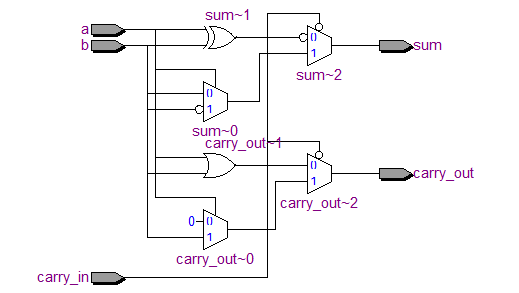
\includegraphics[scale=0.7]{pictures/Oevelse1/Full_adder/Behavioral_RTL.JPG}
		\caption{Full-adder - Behavioral RTL view}
		\label{fig:FaBehavioralRTL}
	\end{figure}
	
	\begin{figure}[h]
		\centering
		\includegraphics[scale=0.7]{pictures/Oevelse1/Full_adder/dataflow_RTL.JPG}
		\caption{Full-adder - Dataflow RTL view}
		\label{fig:FaDataflowRTL}	
	\end{figure}
	
	\begin{figure}[h]
		\centering
		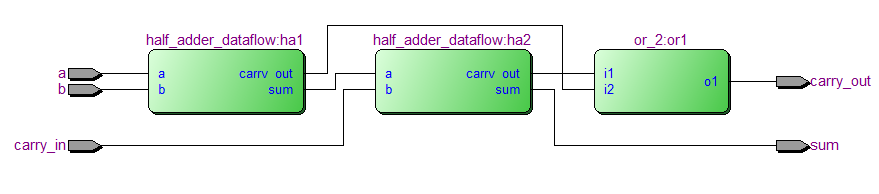
\includegraphics[scale=0.7]{pictures/Oevelse1/Full_adder/Structural_RTL.JPG}
		\caption{Full-adder - Structural RTL view}
		\label{fig:FaStructuralRTL}	
	\end{figure}
	
	\newpage
	\flushleft
		\item[3)]
		Til sidst laver vi en functional simulering for at se om vores tre full-adder koder opfører sig som vi ønsker.\\	

	\begin{figure}[h]
		\centering
		\includegraphics[scale=0.8]{pictures/Oevelse1/Full_adder/Dataflow_functional_simulation.jpg}
		\caption{Full-adder - Dataflow functional Simulation}
		\label{fig:FaDataflowFunctionalSim}
	\end{figure}
	\begin{figure}[h]
		\centering
		\includegraphics[scale=0.8]{pictures/Oevelse1/Full_adder/Behavioral_functional_simulation.jpg}
		\caption{Full-adder - Behavioral functional Simulation}
		\label{fig:FaBehavioralFunctionalSim}
	\end{figure}
	\begin{figure}[h]
		\centering
		\includegraphics[scale=0.6]{pictures/Oevelse1/Full_adder/Structural_functional_simulation.jpg}
		\caption{Full-adder - Structural functional Simulation}
		\label{fig:FaStructuralFunctionalSim}
	\end{figure}
	\newpage

\end{enumerate}


\newpage
\chapter{Øvelse 3}
\section{Opgave 1 - Binary circular watch}
\begin{enumerate}
	\item[1)]
	Vi skriver koden for vores cirkulære ur som det ses i kode \ref{lst:Watch}.\\
	\begin{lstlisting}[caption={VHDL code for binary circular watch},label={lst:Watch}]
	library ieee;
	use ieee.std_logic_1164.all;
	use ieee.numeric_std.all;
	
	entity watch is
	port( clk, speed, reset : in std_logic;
	mode : in std_logic_vector(1 downto 0);
	seg1 : out std_logic_vector(6 downto 0);
	cout : out std_logic);
	bin_val : out std_logic_vector(3 downto 0));
	end watch;
	
	architecture clock of watch is
	
	begin
	u2: entity work.counter port map(clk => clk_out, reset => reset, mode => mode, seg => seg1, cout => cout, bin_val => bin_val);
	
	
	process (reset, clk)
	variable clk_count : integer range 0 to 50000000;
	begin
	if reset = '0' then
	clk_count := 0;
	cout <= '0';
	elsif rising_edge(clk) then
	clk_count := clk_count + 1;
	cout <= '0';
	if speed = '1' then
	if clk_count >= 50000000 then
	cout <= '1';
	clk_count := 0;
	end if;
	elsif speed = '0' then
	if clk_count >= 25000 then
	cout <= '1';
	clk_count := 0;
	end if;
	end if;
	end if;
	
	end process;
	
	end clock;
	
	\end{lstlisting}
	
	Koden for vores counter er illustreret i kode \ref{lst:Counter}
	
		\begin{lstlisting}[caption={VHDL code for binary circular counter},label={lst:Counter}]
		library ieee;
		use ieee.std_logic_1164.all;
		use ieee.numeric_std.all;
		
		entity counter is
		port( clk, reset : in std_logic;
		mode : in std_logic_vector(1 downto 0);
		bin_val : out std_logic_vector(3 downto 0);
		cout : out std_logic;
		seg : out std_logic_vector(6 downto 0));	
		end counter;
		
		architecture circular of counter is
		signal bin_val_sig : std_logic_vector(3 downto 0);
		signal cout_sig : std_logic;
		begin
		
		u1: entity work.BCDdecoder port map(dcba => bin_val_sig, seg => seg);
		
		process (clk, reset, mode, bin_val_sig)
		
		begin
		if reset = '0' then
		bin_val_sig <= "0000";
		cout_sig <= '0';
		elsif rising_edge(clk) then
		if mode = "00" then
		if bin_val_sig = "1001" then 
		bin_val_sig <= "0000";
		cout_sig <= '1';
		else
		bin_val_sig <= std_logic_vector(unsigned(bin_val_sig)+1);
		cout_sig <= '0';
		end if;
		elsif mode = "01" then
		if bin_val_sig = "0101" then 
		bin_val_sig <= "0000";
		cout_sig <= '1';
		else
		bin_val_sig <= std_logic_vector(unsigned(bin_val_sig)+1);
		cout_sig <= '0';
		end if;
		else 
		if bin_val_sig = "0010" then 
		bin_val_sig <= "0000";
		cout_sig <= '1';
		else
		bin_val_sig <= std_logic_vector(unsigned(bin_val_sig)+1);
		cout_sig <= '0';
		end if;
		end if;
		
		end if;
		
		end process;
		bin_val <= bin_val_sig;
		cout <= cout_sig;
		end circular;
		
		\end{lstlisting}
		
		Vi har her anvendt endnu en VHDL-fil kaldet BCD-decoder, som vi i tidligere øvelser har anvendt til at decode vores værdier til visning på et 7-segment display.
		
		Da uret skal kunne tælle op for hvert 5. milisekund i speed-mode, skal counteren kun nå til 25000, som det ses i linje 34.
		
\item[2)] Vi tester vores watch på DE2-boardet. På følgende billeder kan forskellige værdier for 7-segment displayet 'hex0' ses:
		\begin{figure}[h]
			\centering
			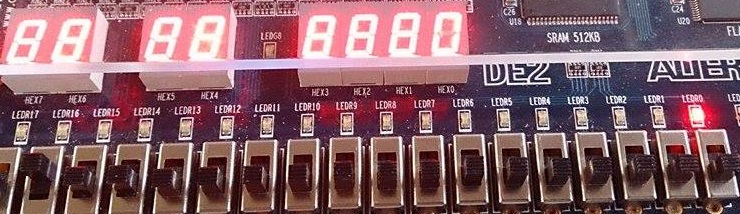
\includegraphics[scale=0.8]{pictures/Oevelse6/opg1/watch0.JPG}
			\caption{Uret er resat}
			\label{fig:alarm0}
		\end{figure}
		
		\begin{figure}[h]
			\centering
			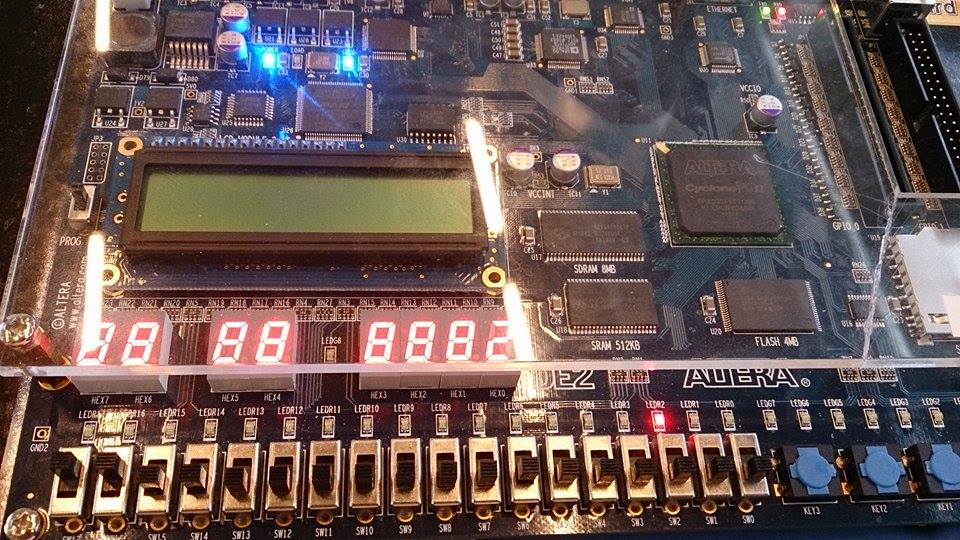
\includegraphics[scale=0.8]{pictures/Oevelse6/opg1/watch2.JPG}
			\caption{Uret viser 2}
			\label{fig:alarm2}
		\end{figure}

		\begin{figure}[h]
			\centering
			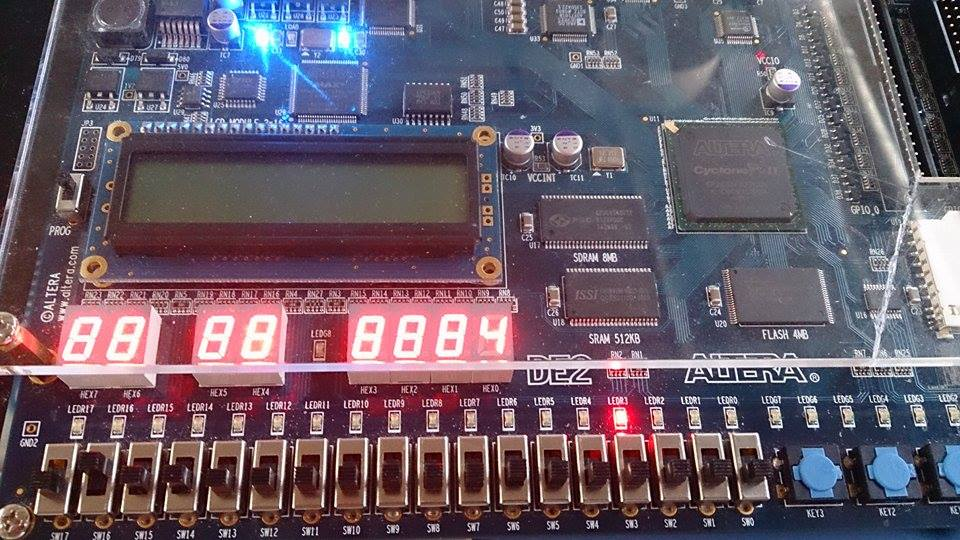
\includegraphics[scale=0.8]{pictures/Oevelse6/opg1/watch4.JPG}
			\caption{Uret viser 4}
			\label{fig:alarm4}
		\end{figure}


\end{enumerate}

\section{Opgave 2 - Full-adder}
	\flushleft
\begin{enumerate}
	\item[1)]
	Med to half-addere kan man lave en full-adder. Dette vil vi nu implementere i hhv. dataflow-style, behavioral-style og structural-style.\\
	\medskip
	\begin{lstlisting}[caption={Full-adder Dataflow VHDL kode},label={lst:FaDataflowCode}]
	library ieee;
	use ieee.std_logic_1164.all;
	
	entity full_adder_dataflow is
	port (a, b, carry_in : in std_logic;
	sum, carry_out : out std_logic);
	end full_adder_dataflow;
	
	architecture dataflow of full_adder_dataflow is
	
	signal s1, s2, s3 : std_logic;
	begin
	s1 <= a xor b; 
	sum <= s1 xor carry_in;
	s2 <= s1 and carry_in;
	s3 <= a and b;
	carry_out <= s2 or s3;
	
	end dataflow;
	\end{lstlisting}
	\medskip
	\begin{lstlisting}[caption={Full-adder Behavioral VHDL kode}, label={lst:FaBehavioralCode}]
	library ieee;
	use ieee.std_logic_1164.all;
	
	entity full_adder_behavioral is
	port (a, b, carry_in : in std_logic;
	sum, carry_out : out std_logic);
	end full_adder_behavioral;
	
	architecture behavioral of full_adder_behavioral is
	
	signal s1, s2, s3 : std_logic;
	begin
	fa: process (carry_in, a, b)
	begin
	if carry_in = '0'  then
	
	if a = '1' then
	sum <= not b;
	carry_out <= b;
	else
	sum <= b;
	carry_out <= '0';
	end if;
	else 
	sum <= a xnor b;
	carry_out <= a or b;
	end if;
	end process fa;
	
	end behavioral;
	\end{lstlisting}
	\medskip
	\begin{lstlisting}[caption={Full-adder Structural VHDL kode},label={lst:FaStructuralCode}]
	library ieee;
	use ieee.std_logic_1164.all;
	
	entity full_adder_structural is
	port (a, b, carry_in : in std_logic;
	sum, carry_out : out std_logic);
	end full_adder_structural;
	
	architecture structural of full_adder_structural is
	
	signal s1, s2, s3 : std_logic;
	begin
	
	ha1: entity work.half_adder_dataflow port map (a => a, b => b, sum => s1, carry_out => s3);
	ha2: entity work.half_adder_dataflow port map (a => s1, b => carry_in, sum => sum, carry_out => s2);
	or1: entity work.or_2 port map (i1 => s2, i2 => s3, o1 => carry_out);
	
	end structural;
	\end{lstlisting}
	\newpage
	\flushleft
		\item[2)]
		Med et RTL view kan vi se hvordan de tre forskellige koder vil blive omdannet til logiske gates.\\
		\begin{figure}[h]
		\centering
		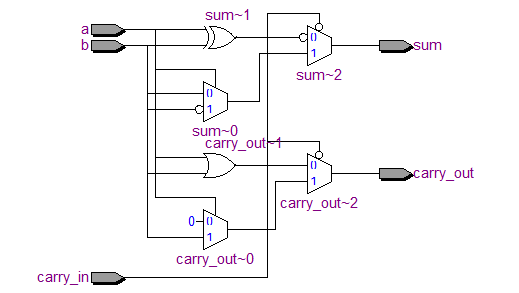
\includegraphics[scale=0.7]{pictures/Oevelse1/Full_adder/Behavioral_RTL.JPG}
		\caption{Full-adder - Behavioral RTL view}
		\label{fig:FaBehavioralRTL}
	\end{figure}
	
	\begin{figure}[h]
		\centering
		\includegraphics[scale=0.7]{pictures/Oevelse1/Full_adder/dataflow_RTL.JPG}
		\caption{Full-adder - Dataflow RTL view}
		\label{fig:FaDataflowRTL}	
	\end{figure}
	
	\begin{figure}[h]
		\centering
		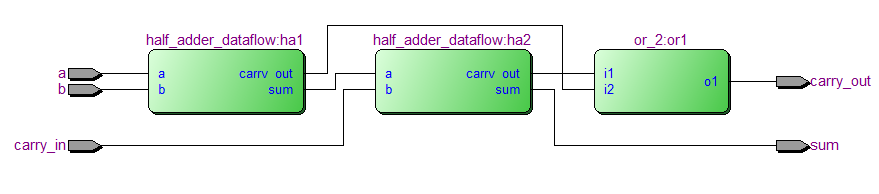
\includegraphics[scale=0.7]{pictures/Oevelse1/Full_adder/Structural_RTL.JPG}
		\caption{Full-adder - Structural RTL view}
		\label{fig:FaStructuralRTL}	
	\end{figure}
	
	\newpage
	\flushleft
		\item[3)]
		Til sidst laver vi en functional simulering for at se om vores tre full-adder koder opfører sig som vi ønsker.\\	

	\begin{figure}[h]
		\centering
		\includegraphics[scale=0.8]{pictures/Oevelse1/Full_adder/Dataflow_functional_simulation.jpg}
		\caption{Full-adder - Dataflow functional Simulation}
		\label{fig:FaDataflowFunctionalSim}
	\end{figure}
	\begin{figure}[h]
		\centering
		\includegraphics[scale=0.8]{pictures/Oevelse1/Full_adder/Behavioral_functional_simulation.jpg}
		\caption{Full-adder - Behavioral functional Simulation}
		\label{fig:FaBehavioralFunctionalSim}
	\end{figure}
	\begin{figure}[h]
		\centering
		\includegraphics[scale=0.6]{pictures/Oevelse1/Full_adder/Structural_functional_simulation.jpg}
		\caption{Full-adder - Structural functional Simulation}
		\label{fig:FaStructuralFunctionalSim}
	\end{figure}
	\newpage

\end{enumerate}


\section{Opgave 3 - Guess a HEX number game}
\begin{enumerate}
	\item[1)]
	Vi skriver koden for vores Guessgame som det ses på figur \ref{lst:Guessgame}.\\
	\begin{lstlisting}[caption={Behavioral style kode for Guessgame},label={lst:Guessgame}]
library ieee;
use ieee.std_logic_1164.all;
use ieee.numeric_std.all;

entity guessgame is 
port (input : in std_logic_vector(7 downto 0);
set, show, try : in std_logic;
seg1, seg10 : out std_logic_vector(6 downto 0));
end guessgame;

architecture game_process of guessgame is
signal i_input10 : std_logic_vector(7 downto 4);
signal i_input1 : std_logic_vector(3 downto 0);
signal i_seg1, i_seg10 : std_logic_vector(3 downto 0);
begin
count: process (set, show, try)

variable target : std_logic_vector(7 downto 0);

begin

--target := "00000000";

if set = '0' then target := input;
elsif show = '0' then 
i_seg1 <= target(3 downto 0);
i_seg10 <= target(7 downto 4);
case i_seg1 is
when "0000" => seg1 <= "0000001"; -- 0
when "0001" => seg1 <= "1001111"; -- 1
when "0010" => seg1 <= "0010010"; -- 2
when "0011" => seg1 <= "0000110"; -- 3
when "0100" => seg1 <= "1001100"; -- 4
when "0101" => seg1 <= "0100100"; -- 5
when "0110" => seg1 <= "0100000"; -- 6
when "0111" => seg1 <= "0001111"; -- 7
when "1000" => seg1 <= "0000000"; -- 8
when "1001" => seg1 <= "0001100"; -- 9
when "1010" => seg1 <= "0001000"; -- A
when "1011" => seg1 <= "1100000"; -- B
when "1100" => seg1 <= "0110001"; -- C
when "1101" => seg1 <= "1000010"; -- D
when "1110" => seg1 <= "0110000"; -- E
when "1111" => seg1 <= "0111000"; -- F
when others => seg1 <= "1111111"; -- Slukket
end case;
case i_seg10 is
when "0000" => seg10 <= "0000001"; -- 0
when "0001" => seg10 <= "1001111"; -- 1
when "0010" => seg10 <= "0010010"; -- 2
when "0011" => seg10 <= "0000110"; -- 3
when "0100" => seg10 <= "1001100"; -- 4
when "0101" => seg10 <= "0100100"; -- 5
when "0110" => seg10 <= "0100000"; -- 6
when "0111" => seg10 <= "0001111"; -- 7
when "1000" => seg10	<= "0000000"; -- 8
when "1001" => seg10	<= "0001100"; -- 9
when "1010" => seg10 <= "0001000"; -- A
when "1011" => seg10 <= "1100000"; -- B
when "1100" => seg10 <= "0110001"; -- C
when "1101" => seg10	<= "1000010"; -- D
when "1110" => seg10 <= "0110000"; -- E
when "1111" => seg10 <= "0111000"; -- F
when others => seg10 <= "1111111"; -- Slukket
end case;
elsif try = '0' then 
if input > target then --output Hi
seg10 <= "1001000"; 
seg1 <= "1111001";
elsif input < target then -- output Lo
seg10 <= "1110001"; 
seg1 <= "1100010";
elsif input = target then -- output --
seg10 <= "1111110"; 
seg1 <= "1111110";
end if;
elsif set = '1' and show = '1' and try = '1' then 
i_input10 <= input(7 downto 4); 
i_input1 <= input(3 downto 0);
case i_input1 is
when "0000" => seg1 <= "0000001"; -- 0
when "0001" => seg1 <= "1001111"; -- 1
when "0010" => seg1 <= "0010010"; -- 2
when "0011" => seg1 <= "0000110"; -- 3
when "0100" => seg1 <= "1001100"; -- 4
when "0101" => seg1 <= "0100100"; -- 5
when "0110" => seg1 <= "0100000"; -- 6
when "0111" => seg1 <= "0001111"; -- 7
when "1000" => seg1 <= "0000000"; -- 8
when "1001" => seg1 <= "0001100"; -- 9
when "1010" => seg1 <= "0001000"; -- A
when "1011" => seg1 <= "1100000"; -- B
when "1100" => seg1 <= "0110001"; -- C
when "1101" => seg1 <= "1000010"; -- D
when "1110" => seg1 <= "0110000"; -- E
when "1111" => seg1 <= "0111000"; -- F
when others => seg1 <= "1111111"; -- Slukket
end case;

case i_input10 is
when "0000" => seg10 <= "0000001"; -- 0
when "0001" => seg10 <= "1001111"; -- 1
when "0010" => seg10 <= "0010010"; -- 2
when "0011" => seg10 <= "0000110"; -- 3
when "0100" => seg10 <= "1001100"; -- 4
when "0101" => seg10 <= "0100100"; -- 5
when "0110" => seg10 <= "0100000"; -- 6
when "0111" => seg10 <= "0001111"; -- 7
when "1000" => seg10 <= "0000000"; -- 8
when "1001" => seg10 <= "0001100"; -- 9
when "1010" => seg10 <= "0001000"; -- A
when "1011" => seg10 <= "1100000"; -- B
when "1100" => seg10 <= "0110001"; -- C
when "1101" => seg10 <= "1000010"; -- D
when "1110" => seg10 <= "0110000"; -- E
when "1111" => seg10 <= "0111000"; -- F
when others => seg10 <= "1111111"; -- Slukket
end case;
end if;
end process count;
end game_process;


	\end{lstlisting}
	\item[2)]
	Vi downloader programmet til vores DE2-board, hvor SW[0-3] vises på HEX0, SW[4-7] vises på HEX1, KEY3 = set, KEY2 = show og KEY1 = try. \\
	\begin{figure}[h]
		\centering
		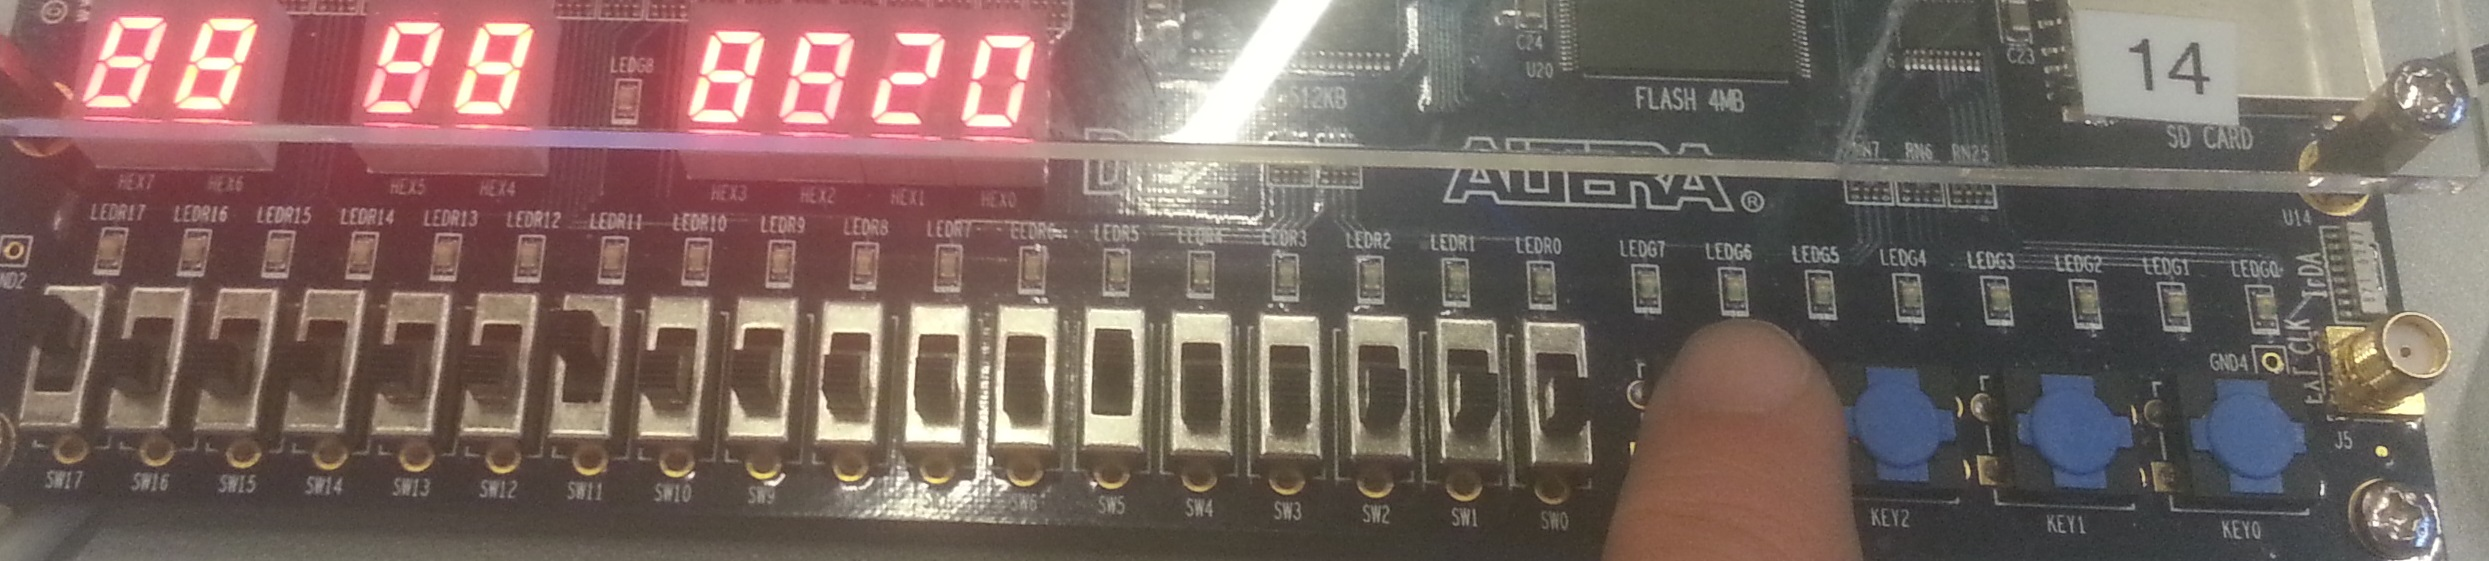
\includegraphics[scale=0.8]{pictures/Oevelse5/opg3/guess_set.JPG}
		\caption{}
		\label{fig:GuessSet}
	\end{figure}
	\begin{figure}[h]
		\centering
		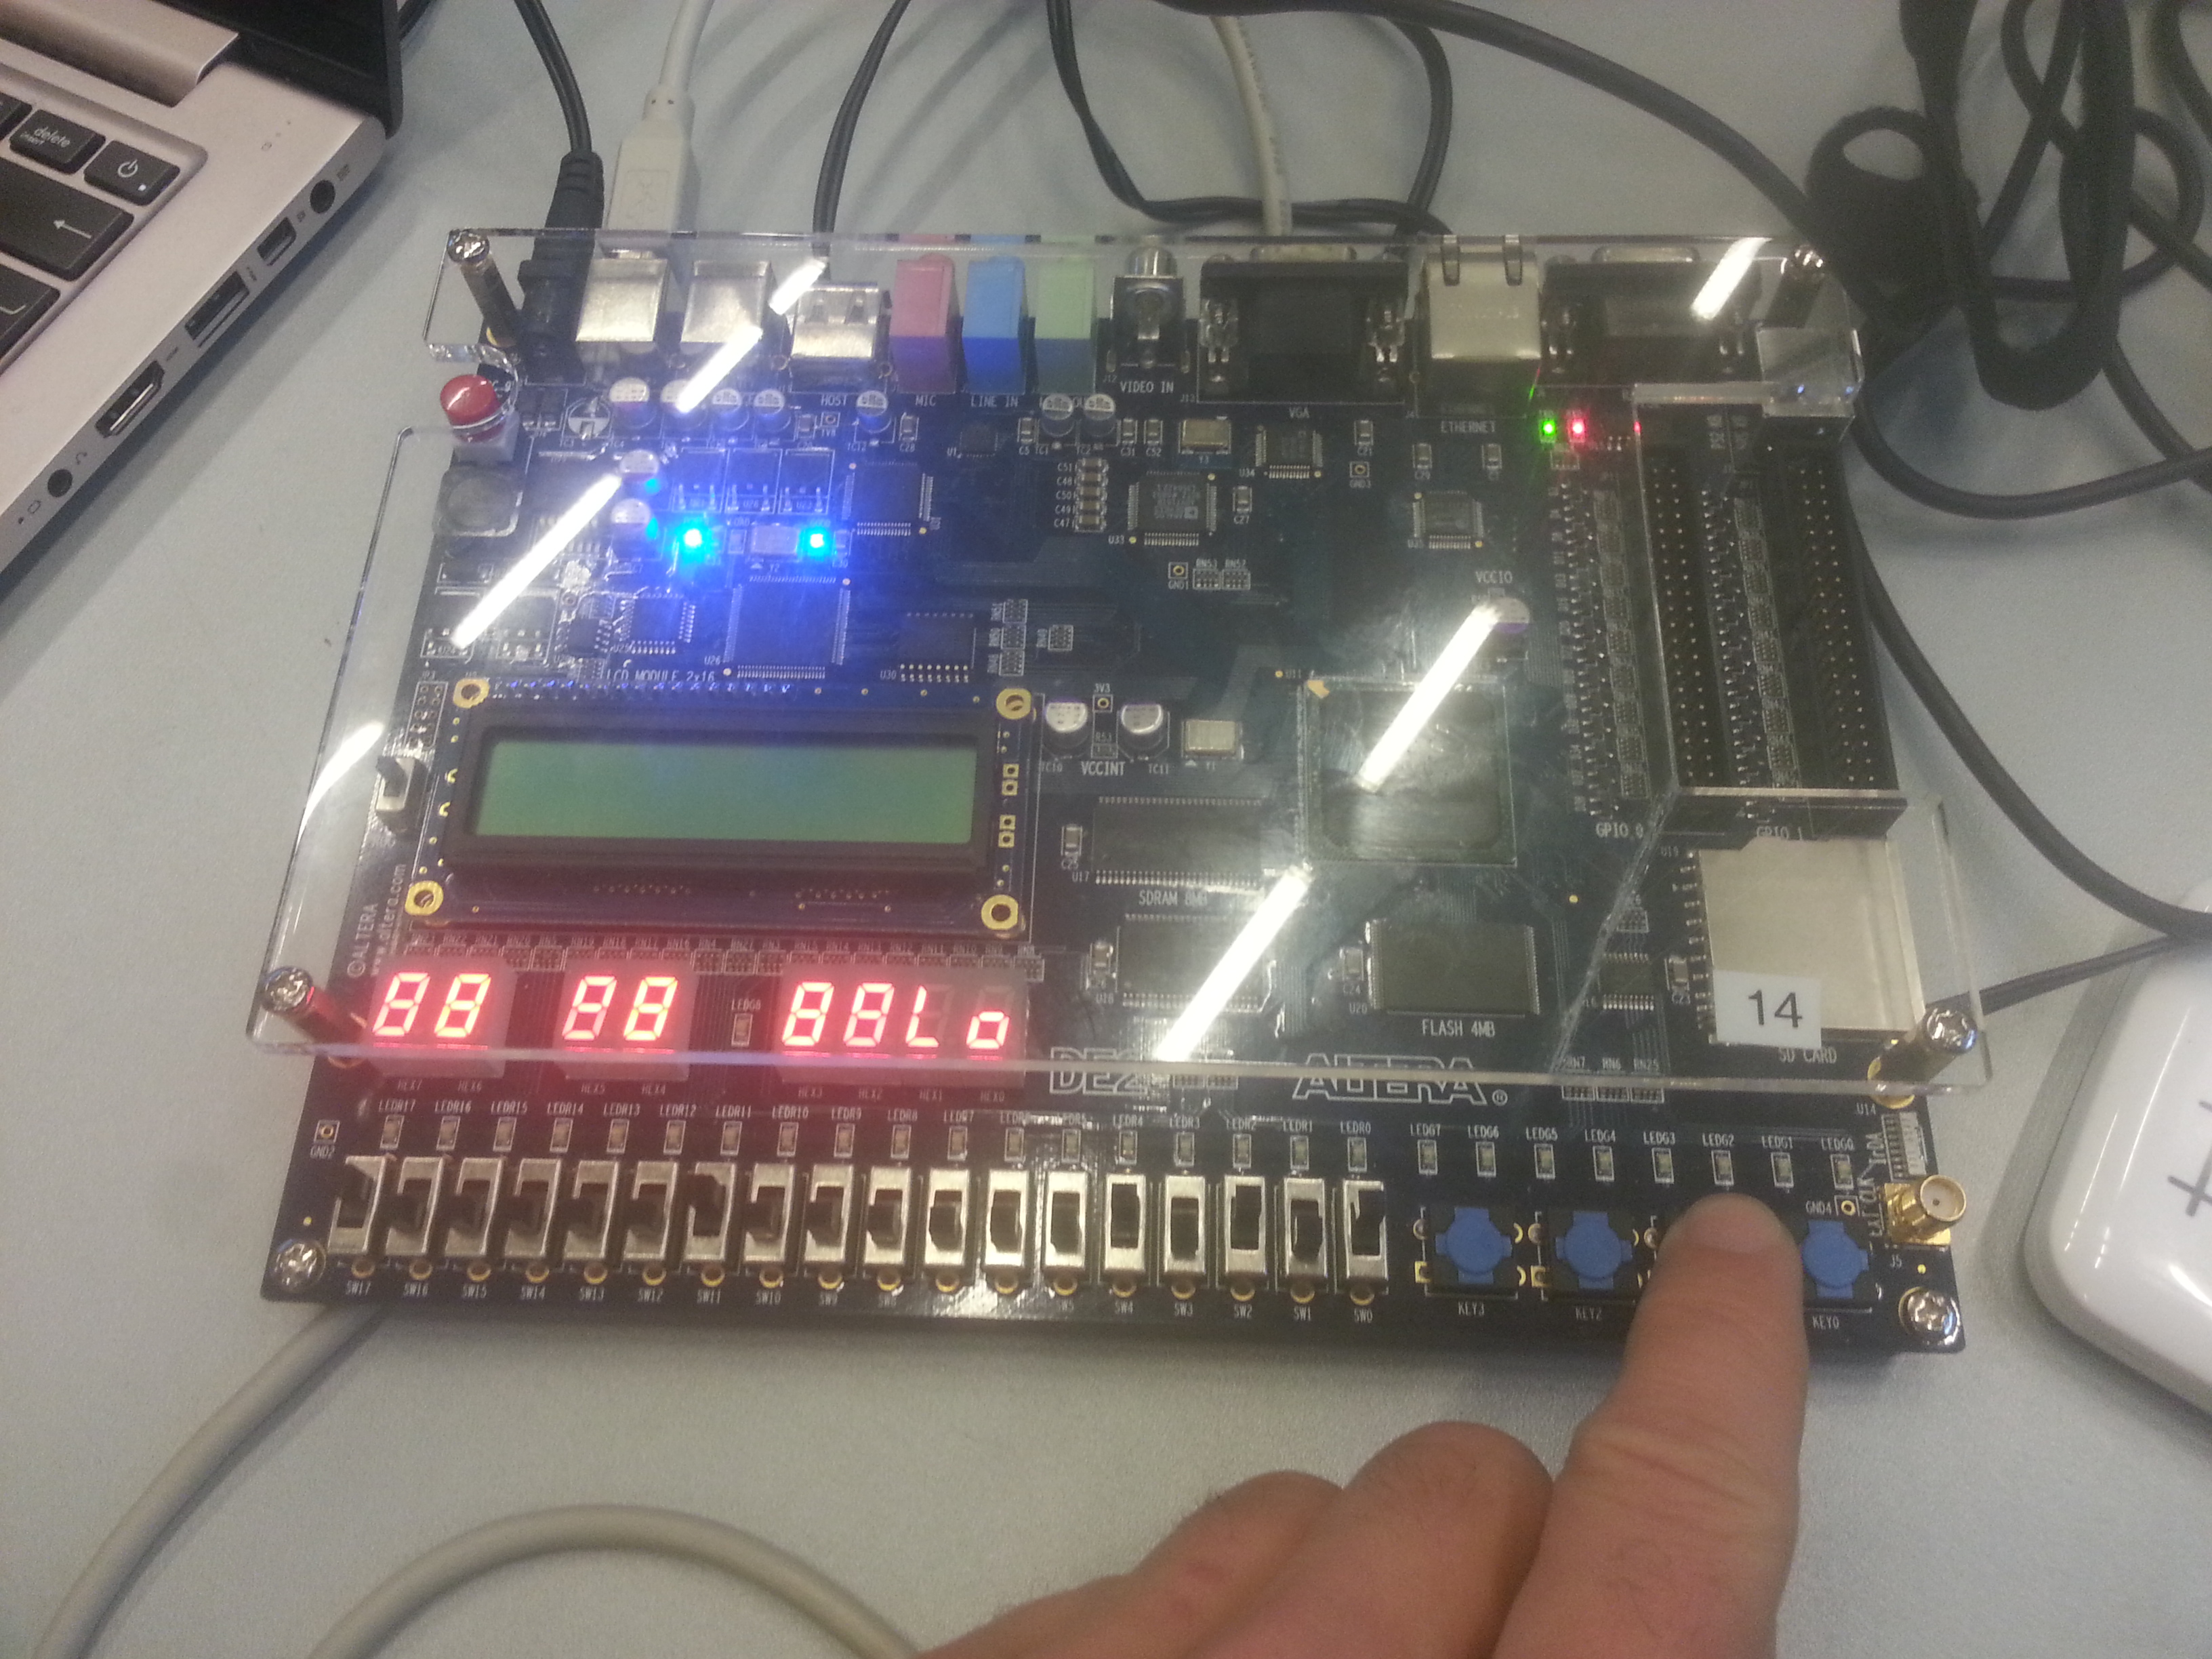
\includegraphics[scale=0.8]{pictures/Oevelse5/opg3/guess_try_lo.JPG}
		\caption{}
		\label{fig:GuessTryLo}
	\end{figure}
	\begin{figure}[h]
		\centering
		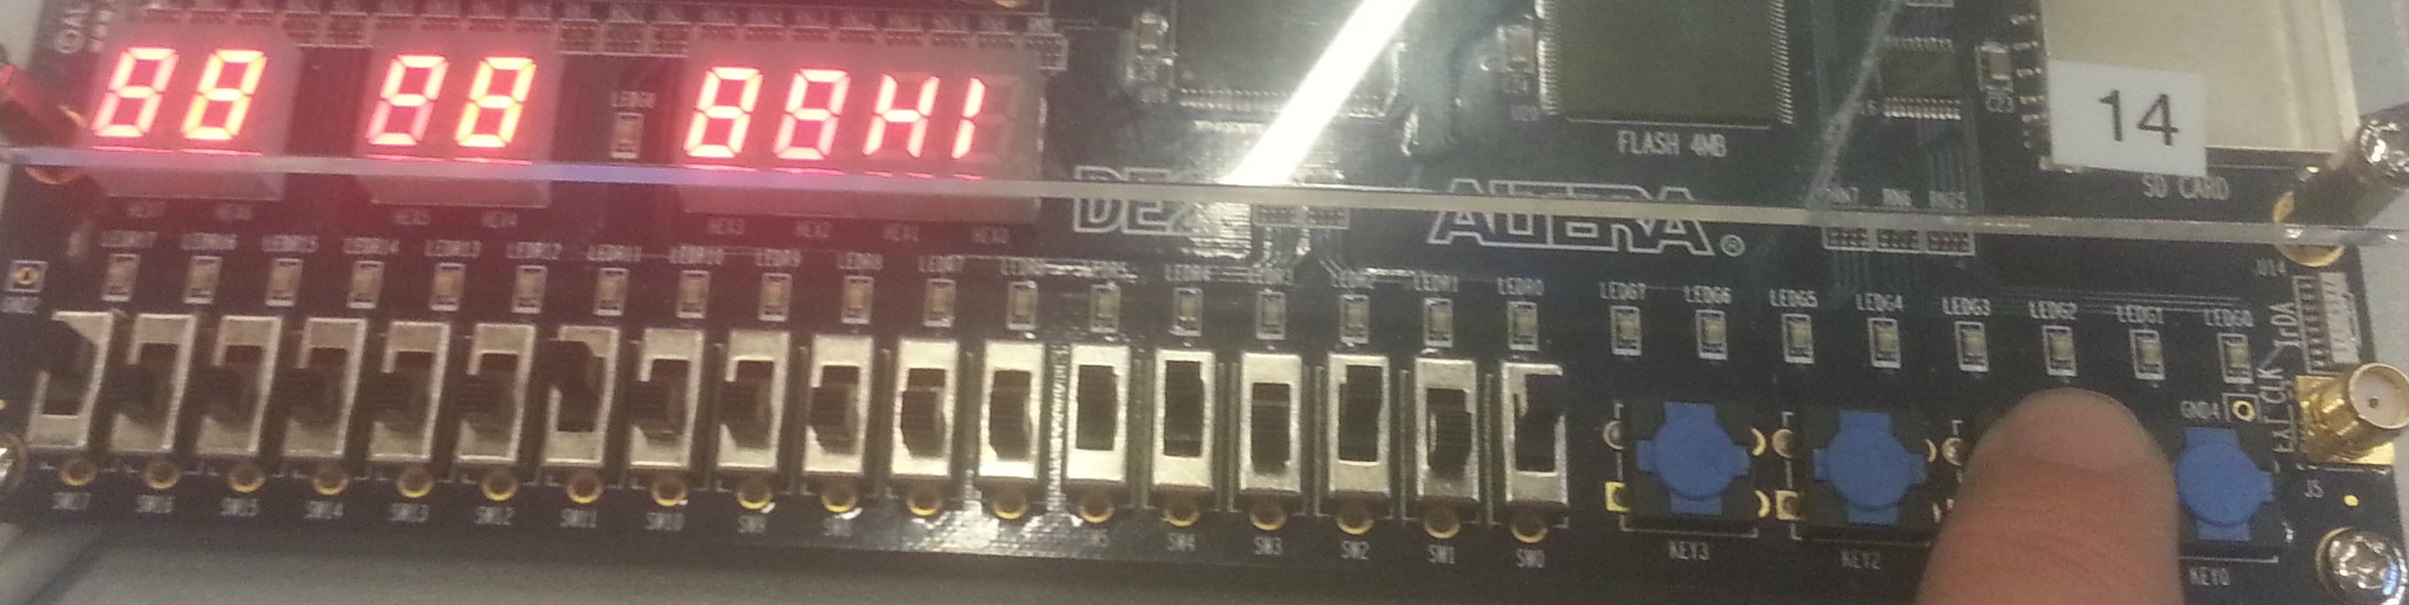
\includegraphics[scale=0.8]{pictures/Oevelse5/opg3/guess_try_hi.JPG}
		\caption{}
		\label{fig:GuessTryHi}
	\end{figure}
	\begin{figure}[h]
		\centering
		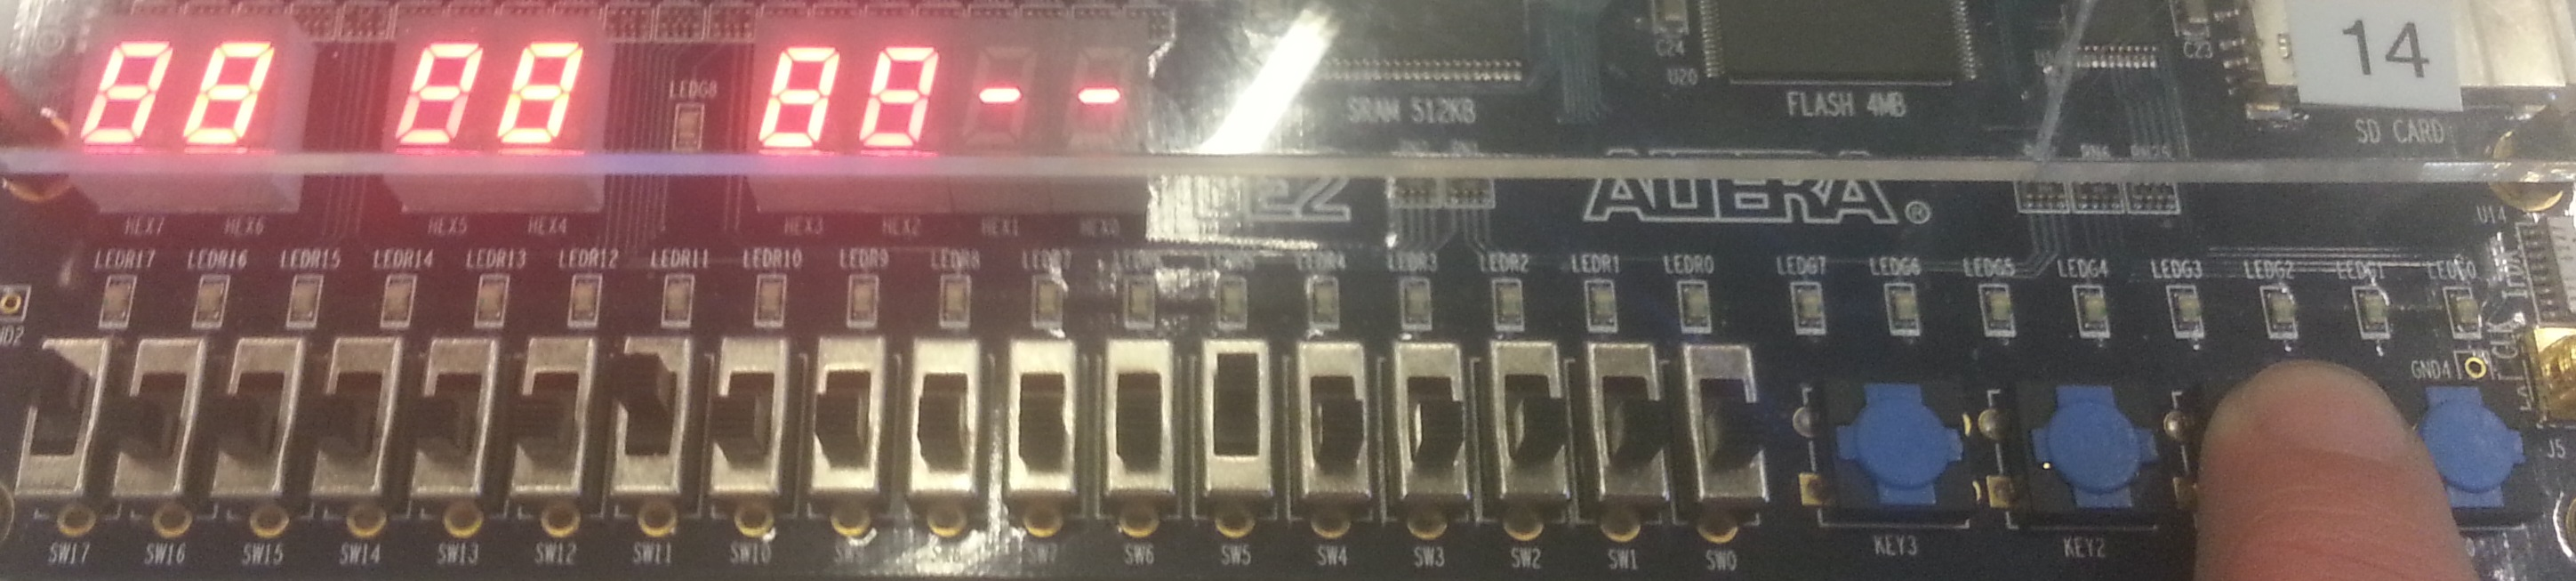
\includegraphics[scale=0.8]{pictures/Oevelse5/opg3/guess_try_ok.JPG}
		\caption{}
		\label{fig:GuessTryOk}
	\end{figure}
	\begin{figure}[h]
		\centering
		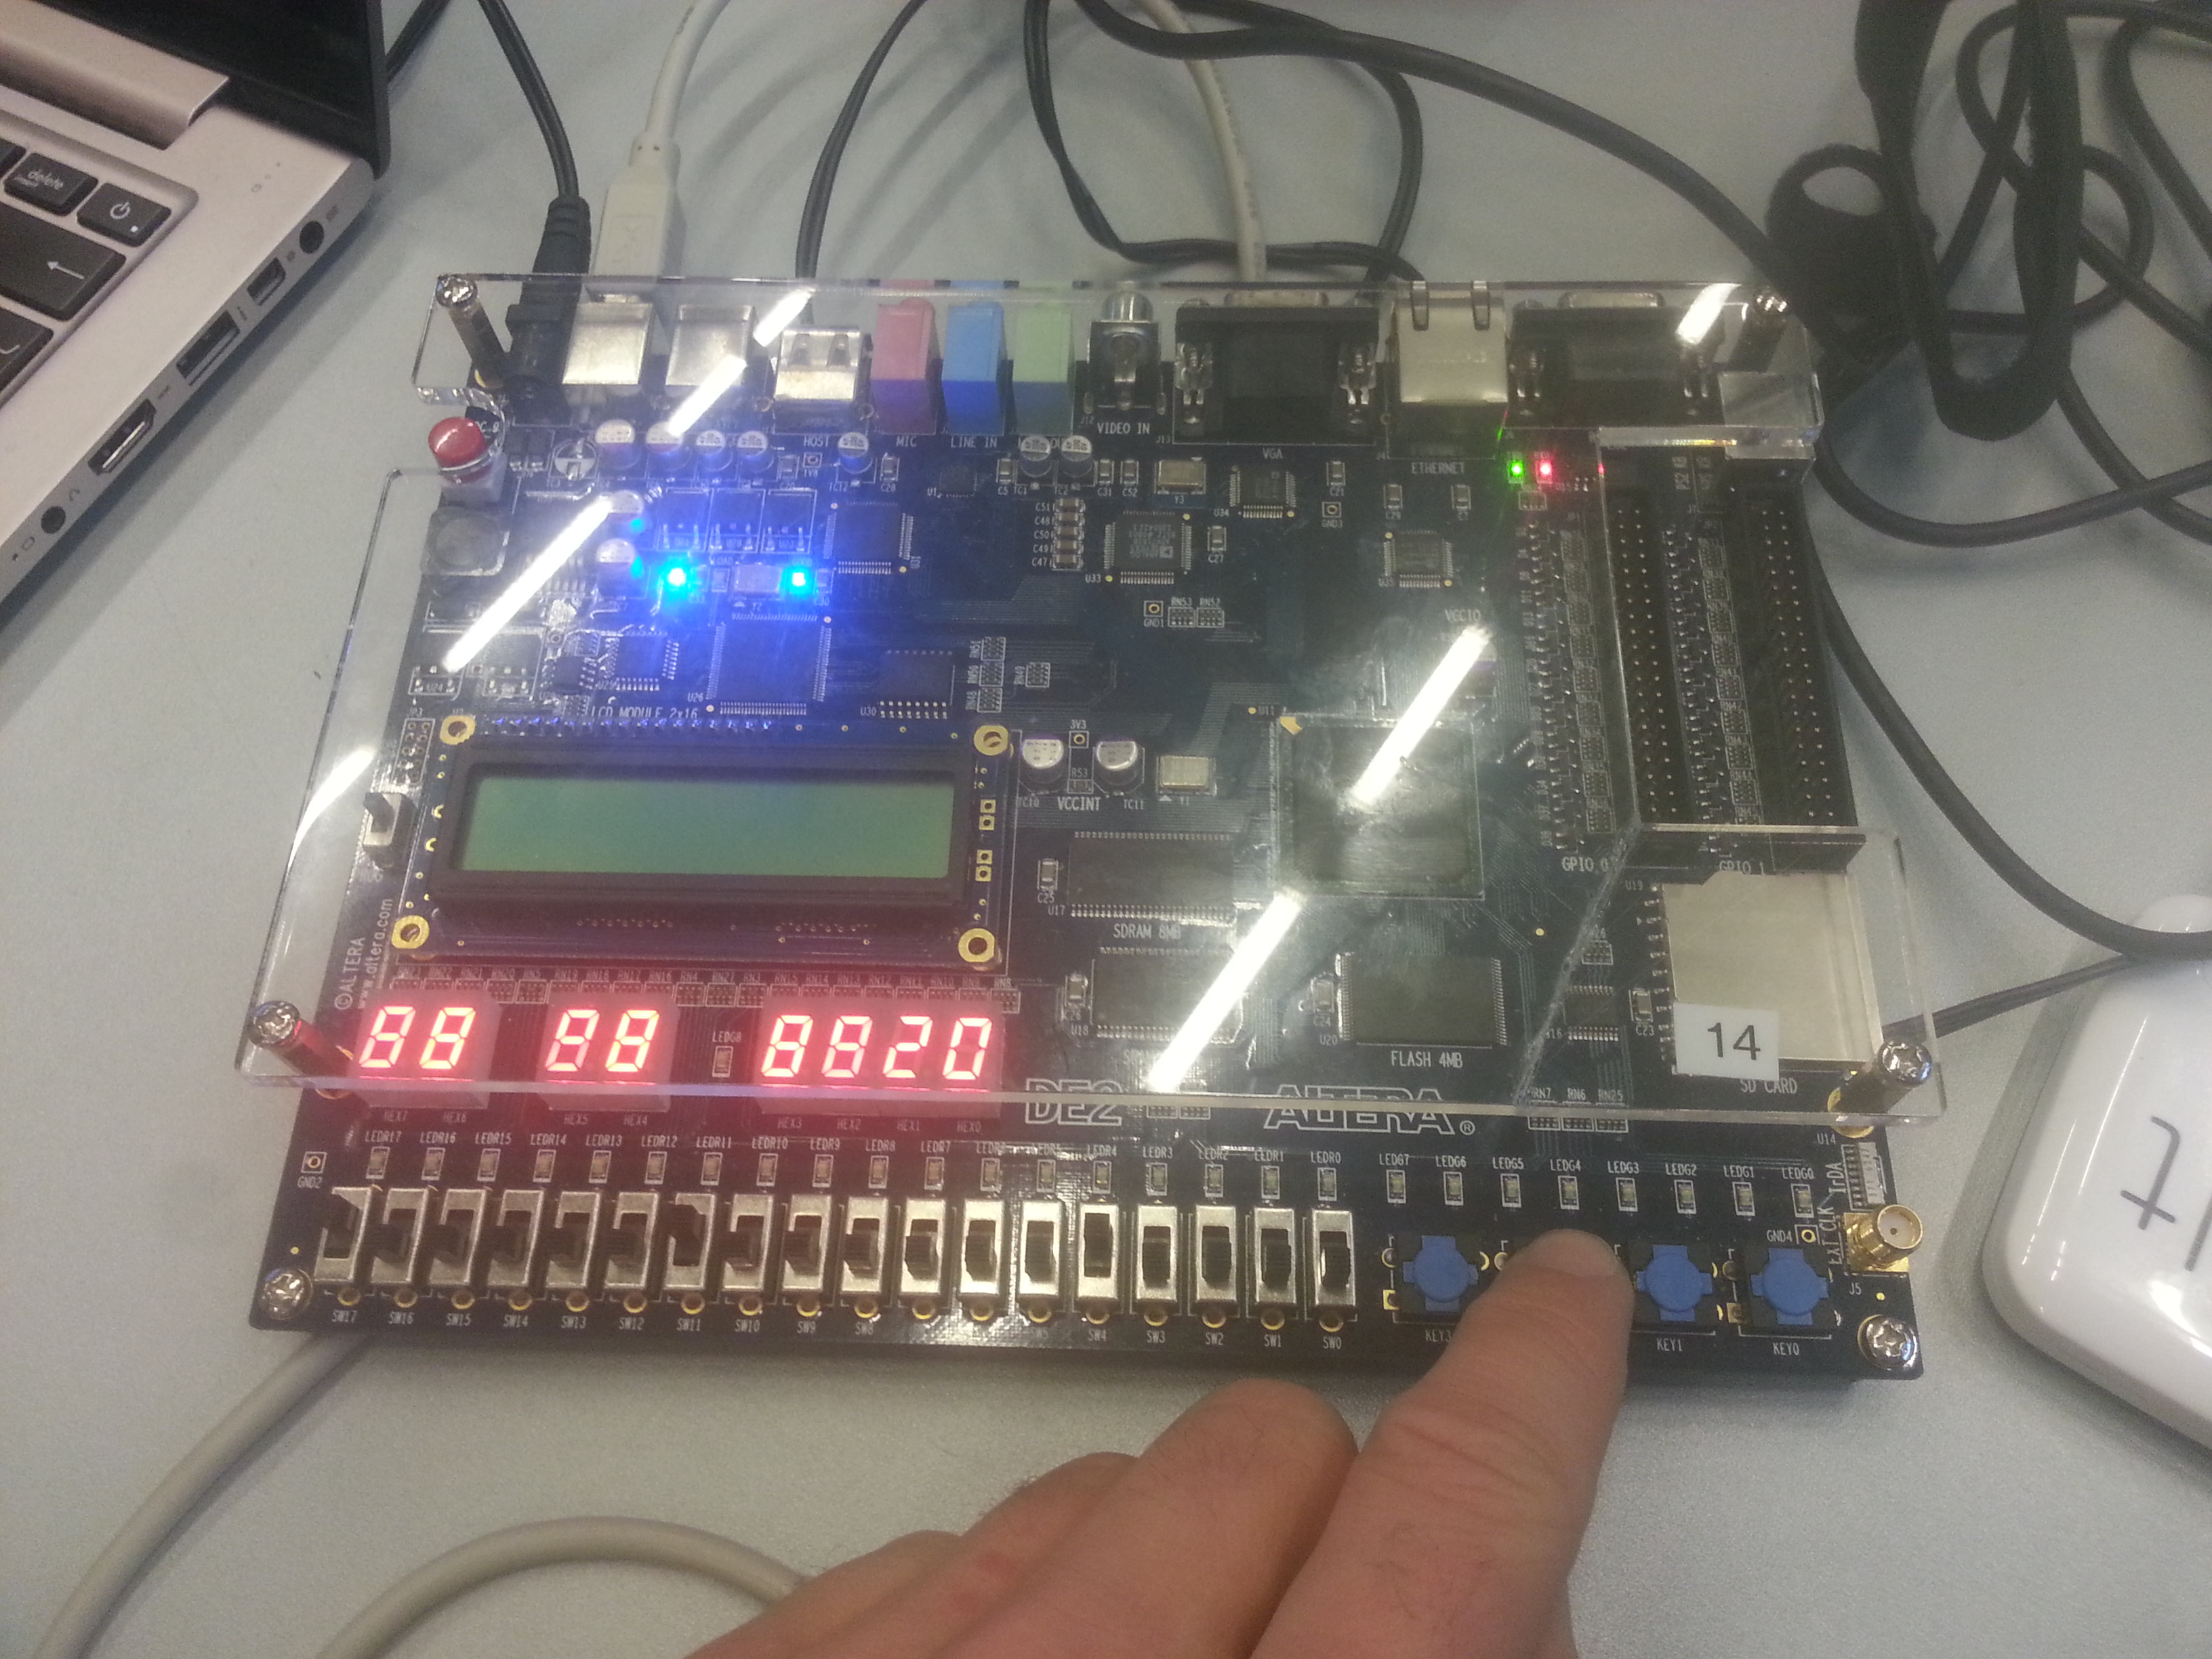
\includegraphics[scale=0.8]{pictures/Oevelse5/opg3/guess_show.JPG}
		\caption{}
		\label{fig:GuessShow}
	\end{figure}
		\item[1)]
		Vi skriver koden for vores Guessgame som det ses på figur \ref{lst:Guessgame}.\\
		\begin{lstlisting}[caption={Behavioral style kode for Guessgame},label={lst:Guessgame}]
		library ieee;
		use ieee.std_logic_1164.all;
		use ieee.numeric_std.all;
		
		entity guessgame is 
		port (input : in std_logic_vector(7 downto 0);
		set, show, try : in std_logic;
		seg1, seg10 : out std_logic_vector(6 downto 0));
		end guessgame;
		
		architecture game_process of guessgame is
		signal i_input10 : std_logic_vector(7 downto 4);
		signal i_input1 : std_logic_vector(3 downto 0);
		signal i_seg1, i_seg10 : std_logic_vector(3 downto 0);
		begin
		count: process (set, show, try)
		
		variable target : std_logic_vector(7 downto 0);
		
		begin
		
		--target := "00000000";
		
		if set = '0' then target := input;
		elsif show = '0' then 
		i_seg1 <= target(3 downto 0);
		i_seg10 <= target(7 downto 4);
		case i_seg1 is
		when "0000" => seg1 <= "0000001"; -- 0
		when "0001" => seg1 <= "1001111"; -- 1
		when "0010" => seg1 <= "0010010"; -- 2
		when "0011" => seg1 <= "0000110"; -- 3
		when "0100" => seg1 <= "1001100"; -- 4
		when "0101" => seg1 <= "0100100"; -- 5
		when "0110" => seg1 <= "0100000"; -- 6
		when "0111" => seg1 <= "0001111"; -- 7
		when "1000" => seg1 <= "0000000"; -- 8
		when "1001" => seg1 <= "0001100"; -- 9
		when "1010" => seg1 <= "0001000"; -- A
		when "1011" => seg1 <= "1100000"; -- B
		when "1100" => seg1 <= "0110001"; -- C
		when "1101" => seg1 <= "1000010"; -- D
		when "1110" => seg1 <= "0110000"; -- E
		when "1111" => seg1 <= "0111000"; -- F
		when others => seg1 <= "1111111"; -- Slukket
		end case;
		case i_seg10 is
		when "0000" => seg10 <= "0000001"; -- 0
		when "0001" => seg10 <= "1001111"; -- 1
		when "0010" => seg10 <= "0010010"; -- 2
		when "0011" => seg10 <= "0000110"; -- 3
		when "0100" => seg10 <= "1001100"; -- 4
		when "0101" => seg10 <= "0100100"; -- 5
		when "0110" => seg10 <= "0100000"; -- 6
		when "0111" => seg10 <= "0001111"; -- 7
		when "1000" => seg10	<= "0000000"; -- 8
		when "1001" => seg10	<= "0001100"; -- 9
		when "1010" => seg10 <= "0001000"; -- A
		when "1011" => seg10 <= "1100000"; -- B
		when "1100" => seg10 <= "0110001"; -- C
		when "1101" => seg10	<= "1000010"; -- D
		when "1110" => seg10 <= "0110000"; -- E
		when "1111" => seg10 <= "0111000"; -- F
		when others => seg10 <= "1111111"; -- Slukket
		end case;
		elsif try = '0' then 
		if input > target then --output Hi
		seg10 <= "1001000"; 
		seg1 <= "1111001";
		elsif input < target then -- output Lo
		seg10 <= "1110001"; 
		seg1 <= "1100010";
		elsif input = target then -- output --
		seg10 <= "1111110"; 
		seg1 <= "1111110";
		end if;
		elsif set = '1' and show = '1' and try = '1' then 
		i_input10 <= input(7 downto 4); 
		i_input1 <= input(3 downto 0);
		case i_input1 is
		when "0000" => seg1 <= "0000001"; -- 0
		when "0001" => seg1 <= "1001111"; -- 1
		when "0010" => seg1 <= "0010010"; -- 2
		when "0011" => seg1 <= "0000110"; -- 3
		when "0100" => seg1 <= "1001100"; -- 4
		when "0101" => seg1 <= "0100100"; -- 5
		when "0110" => seg1 <= "0100000"; -- 6
		when "0111" => seg1 <= "0001111"; -- 7
		when "1000" => seg1 <= "0000000"; -- 8
		when "1001" => seg1 <= "0001100"; -- 9
		when "1010" => seg1 <= "0001000"; -- A
		when "1011" => seg1 <= "1100000"; -- B
		when "1100" => seg1 <= "0110001"; -- C
		when "1101" => seg1 <= "1000010"; -- D
		when "1110" => seg1 <= "0110000"; -- E
		when "1111" => seg1 <= "0111000"; -- F
		when others => seg1 <= "1111111"; -- Slukket
		end case;
		
		case i_input10 is
		when "0000" => seg10 <= "0000001"; -- 0
		when "0001" => seg10 <= "1001111"; -- 1
		when "0010" => seg10 <= "0010010"; -- 2
		when "0011" => seg10 <= "0000110"; -- 3
		when "0100" => seg10 <= "1001100"; -- 4
		when "0101" => seg10 <= "0100100"; -- 5
		when "0110" => seg10 <= "0100000"; -- 6
		when "0111" => seg10 <= "0001111"; -- 7
		when "1000" => seg10 <= "0000000"; -- 8
		when "1001" => seg10 <= "0001100"; -- 9
		when "1010" => seg10 <= "0001000"; -- A
		when "1011" => seg10 <= "1100000"; -- B
		when "1100" => seg10 <= "0110001"; -- C
		when "1101" => seg10 <= "1000010"; -- D
		when "1110" => seg10 <= "0110000"; -- E
		when "1111" => seg10 <= "0111000"; -- F
		when others => seg10 <= "1111111"; -- Slukket
		end case;
		end if;
		end process count;
		end game_process;
		
		
		\end{lstlisting}
		\item[2)]
		Vi downloader programmet til vores DE2-board, hvor SW[0-3] vises på HEX0, SW[4-7] vises på HEX1, KEY3 = set, KEY2 = show og KEY1 = try. \\
		\begin{figure}[h]
			\centering
			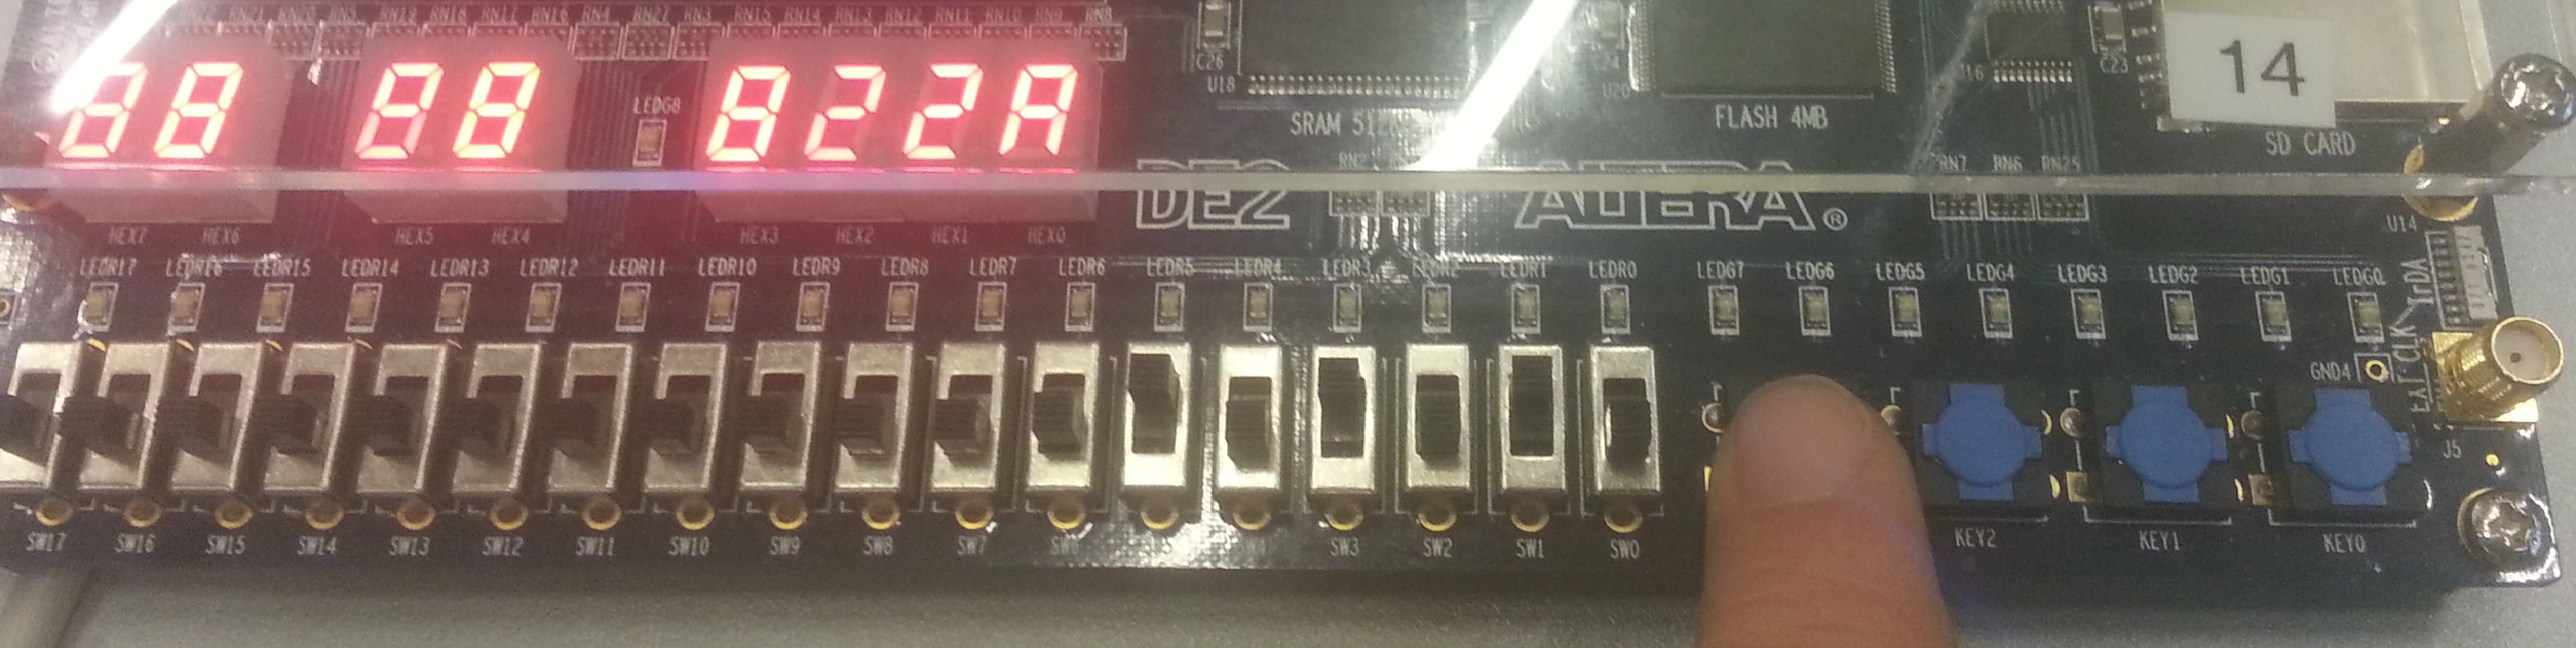
\includegraphics[scale=0.15]{pictures/Oevelse5/opg3/guess_2p_set.JPG}
			\caption{Tal sættes af player 2}
			\label{fig:Guess2pSet}
		\end{figure}
		\begin{figure}[h]
			\centering
			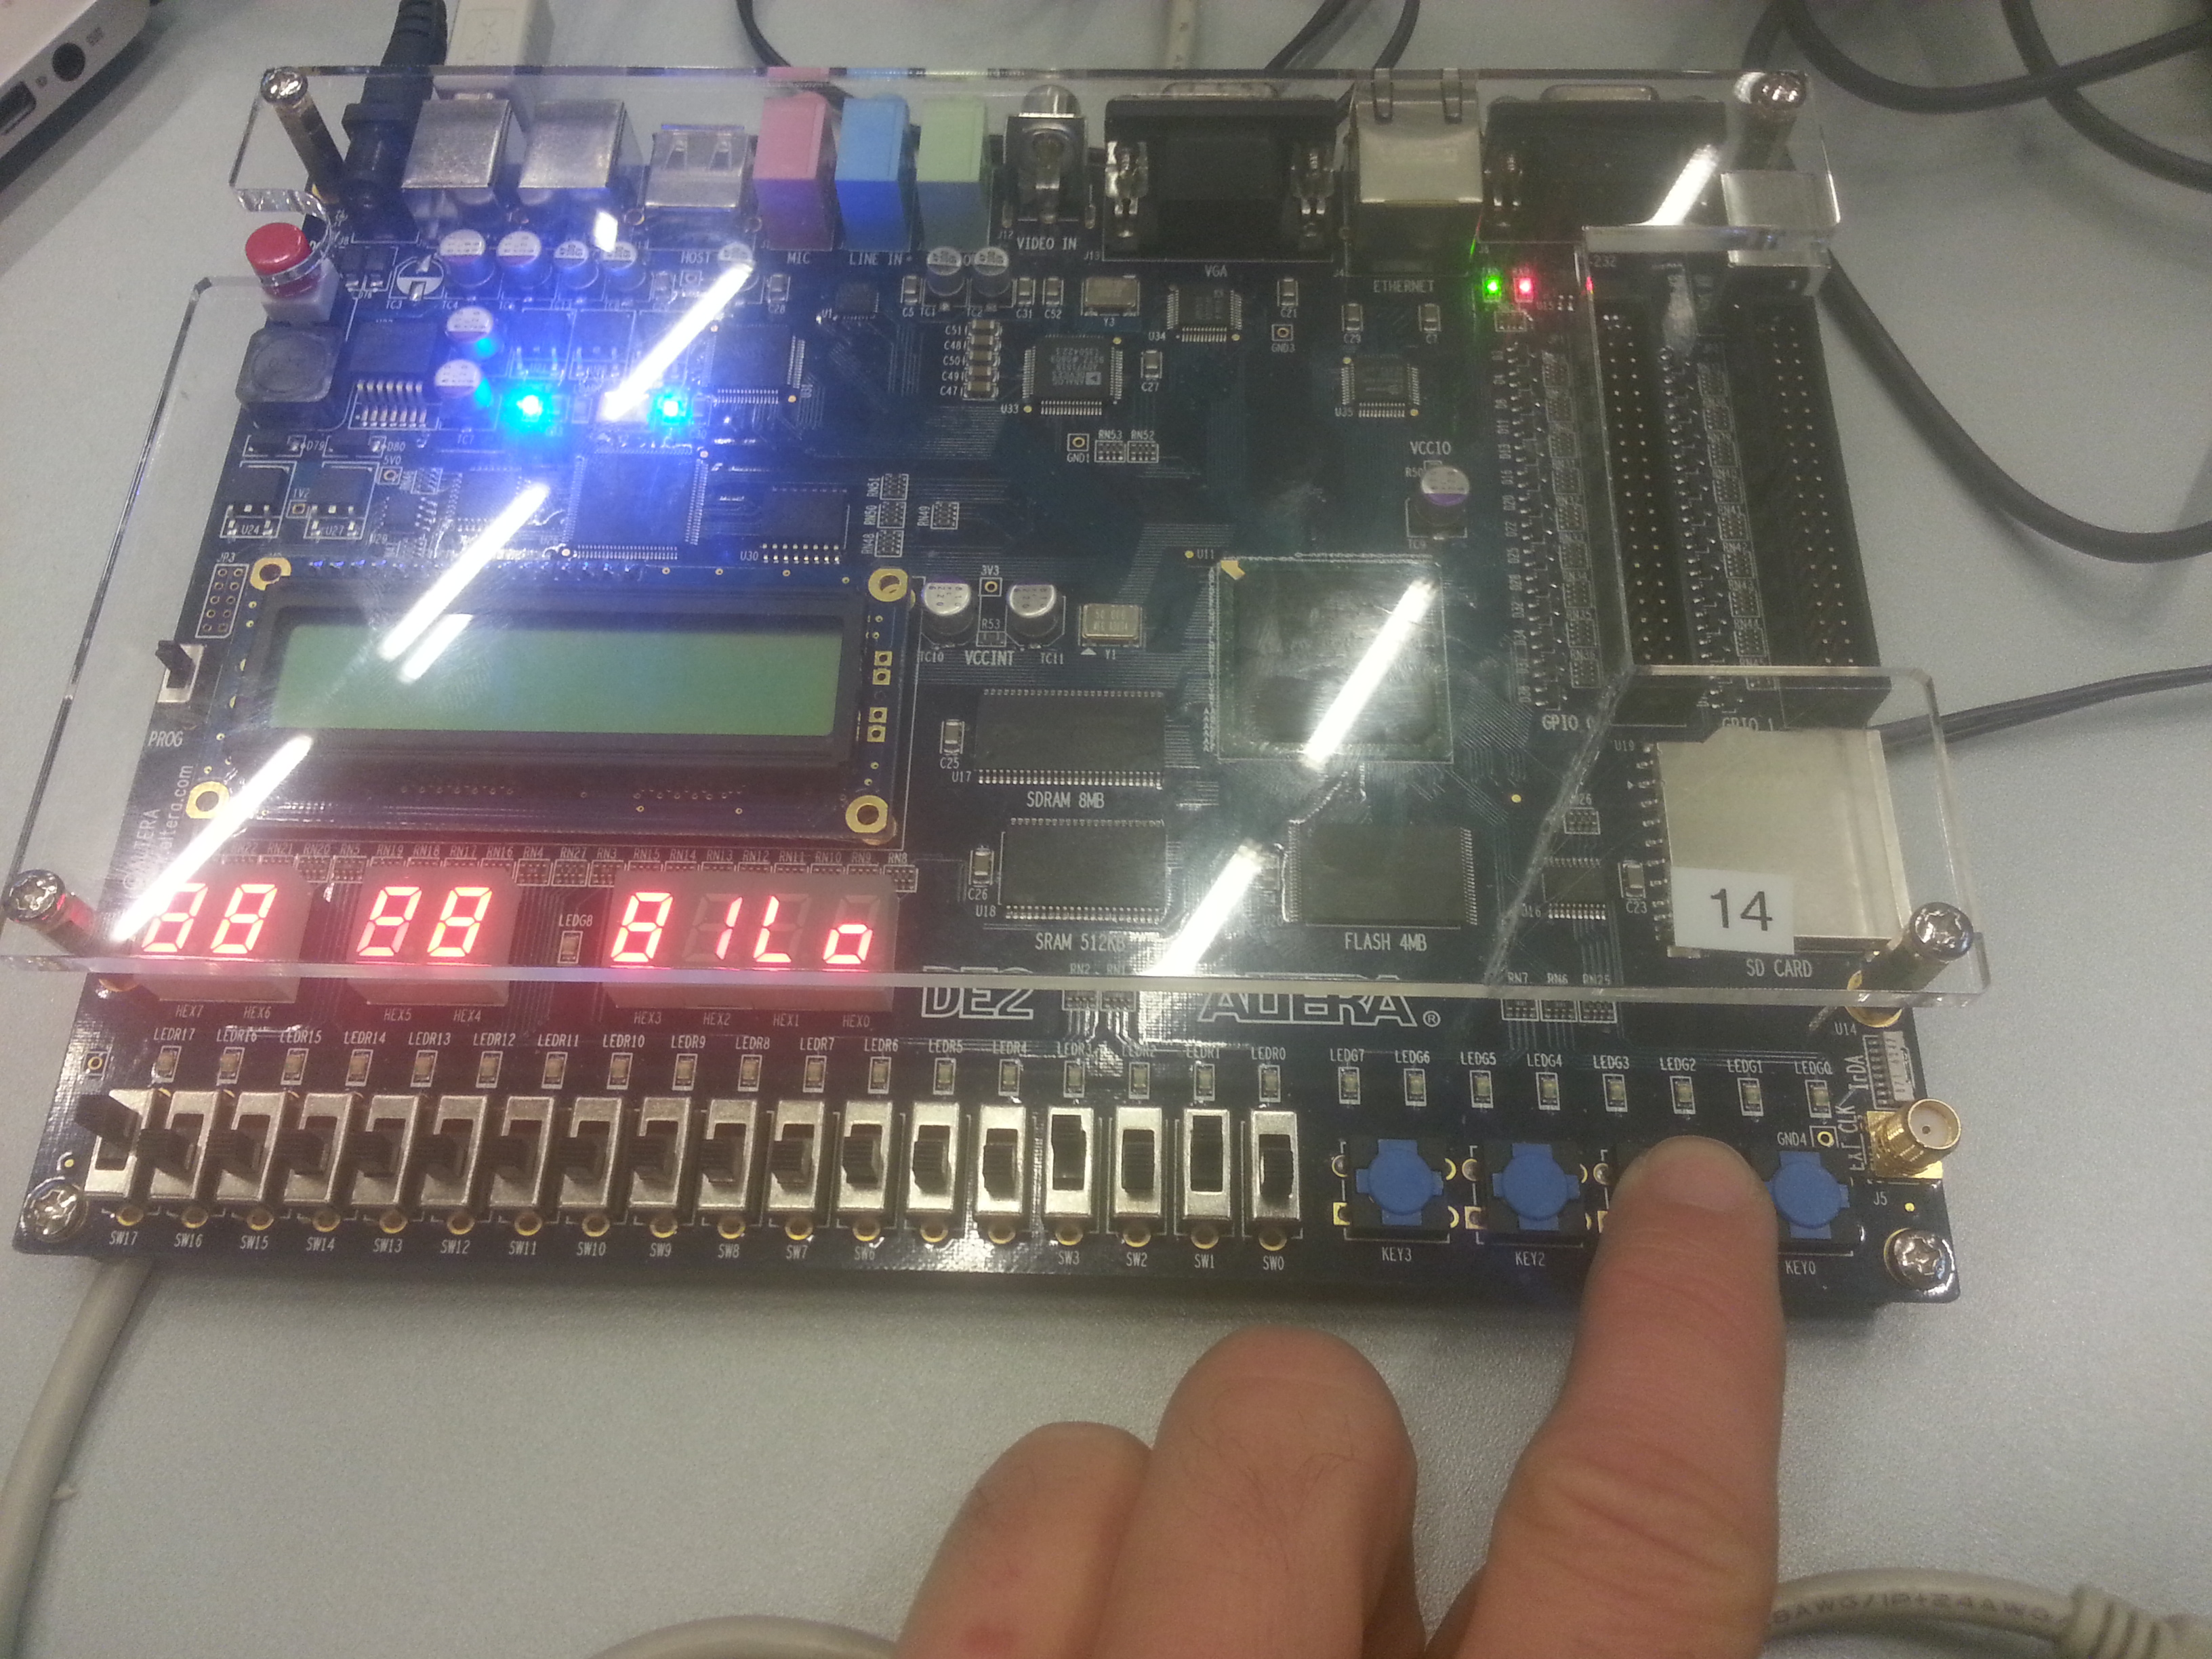
\includegraphics[scale=0.15]{pictures/Oevelse5/opg3/guess_2p_try_lo.JPG}
			\caption{Tal gættes af player 1 og findes for lavt}
			\label{fig:Guess2pTryLo}
		\end{figure}
		\begin{figure}[h]
			\centering
			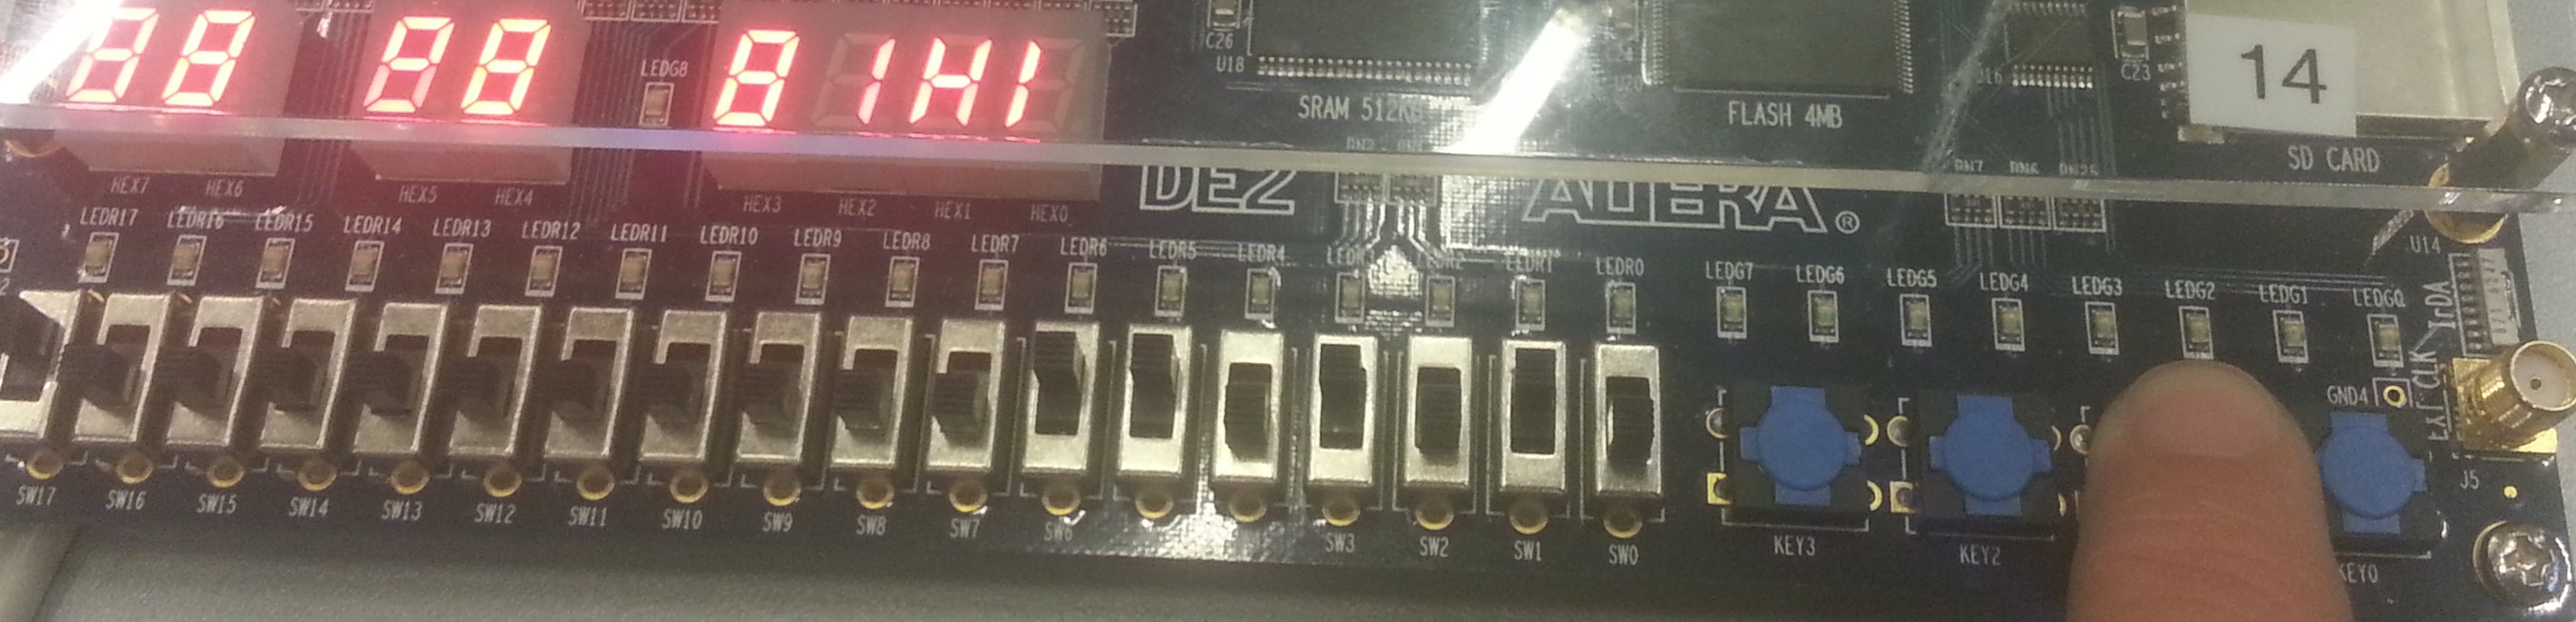
\includegraphics[scale=0.15]{pictures/Oevelse5/opg3/guess_2p_try_hi.JPG}
			\caption{Tal gættes af player 1 og findes for højt}
			\label{fig:Guess2pTryHi}
		\end{figure}
		\begin{figure}[h]
			\centering
			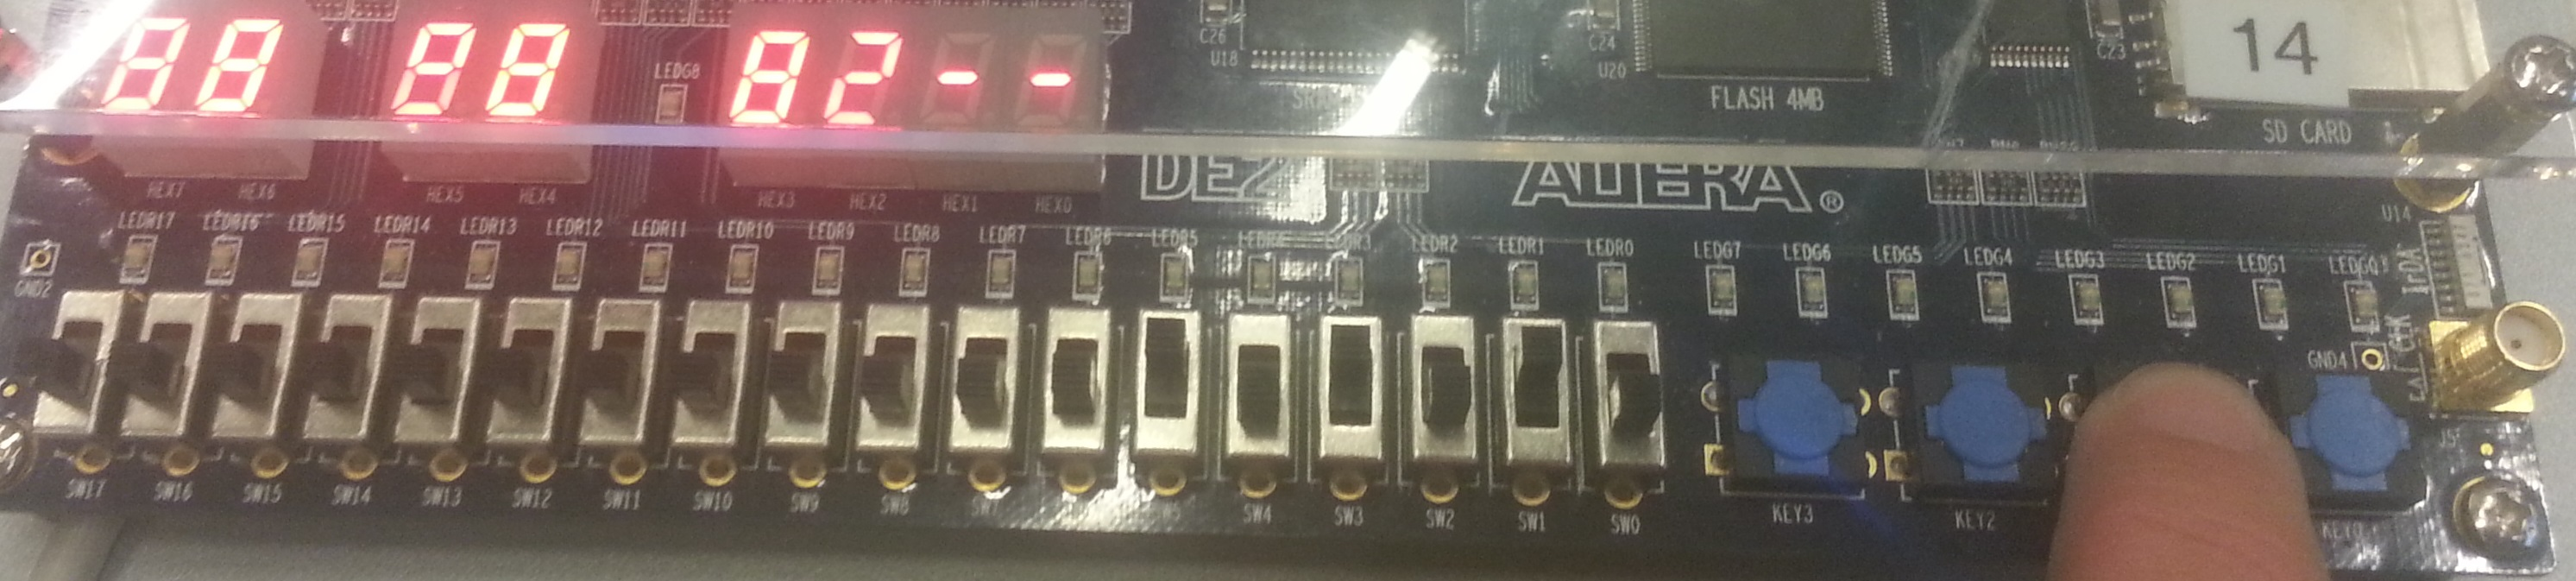
\includegraphics[scale=0.15]{pictures/Oevelse5/opg3/guess_2p_try_ok.JPG}
			\caption{Tal gættes af player 2 og er korrekt}
			\label{fig:Guess2pTryOk}
		\end{figure}
		\begin{figure}[h]
			\centering
			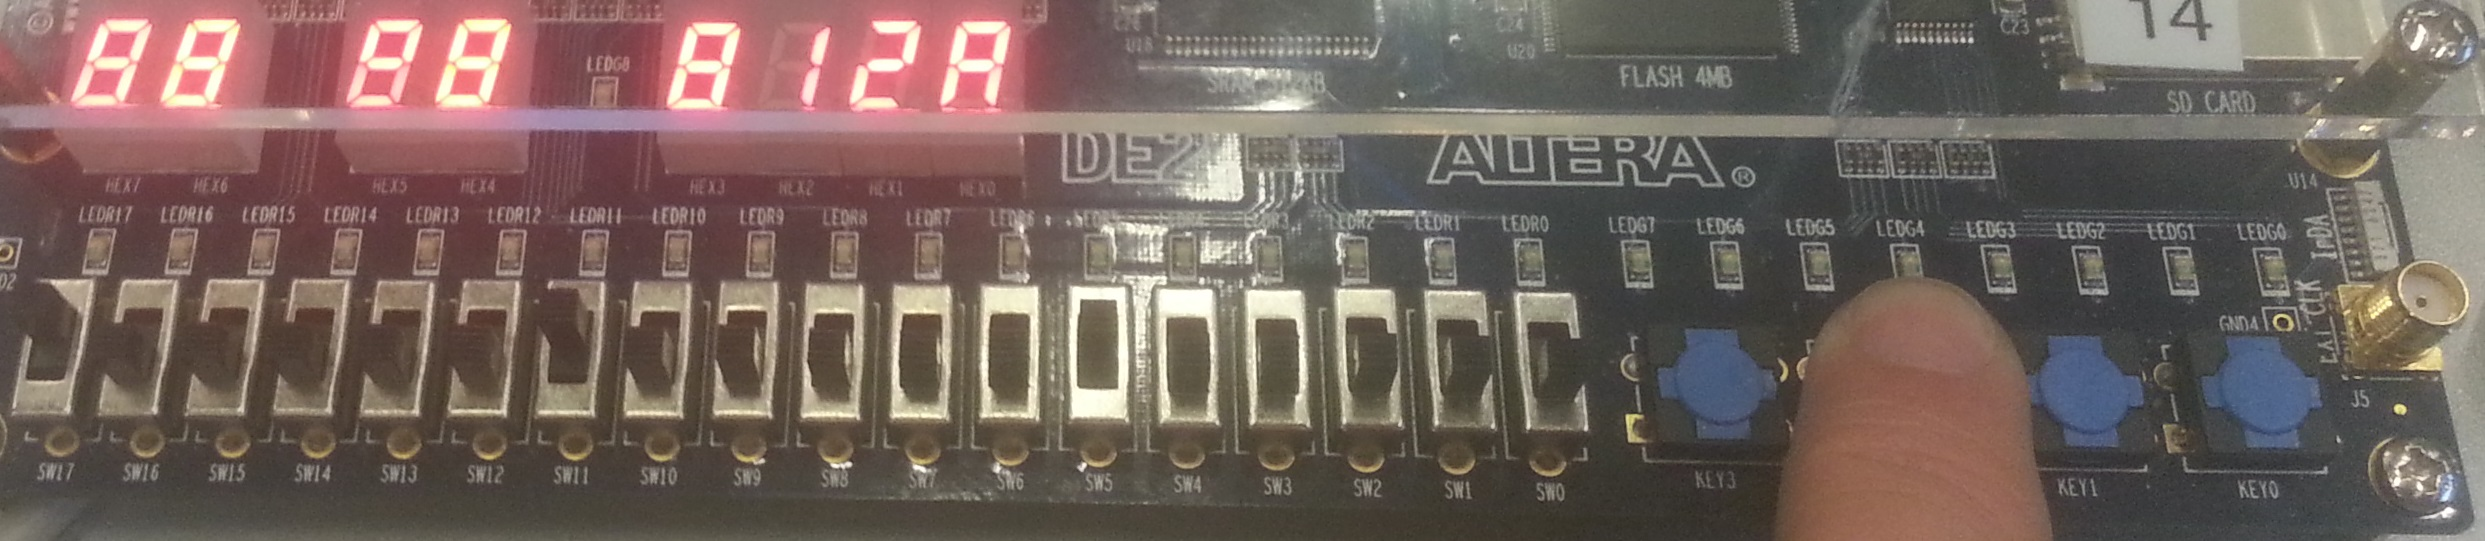
\includegraphics[scale=0.15]{pictures/Oevelse5/opg3/guess_2p_show.JPG}
			\caption{Player 1 viser gemte tal}
			\label{fig:Guess2pShow}
		\end{figure}
\end{enumerate}
\section{Opgave 4 - 8 input NAND using the for loop}
\begin{enumerate}
	\item[1)]
	Vi skriver koden for en 8 input NAND gate ved hjælp af en for løkke i behavioral style som det ses på figur \ref{lst:8innand}.\\
	\begin{lstlisting}[caption={Behavioral style kode for en 8 input NAND gate},label={lst:8innand}]
	library ieee;
	use ieee.std_logic_1164.all;
	
	entity inNAND is
	port (input : in std_logic_vector(7 downto 0);
	nand_8 : out std_logic);
	end inNAND;
	
	architecture nand_process of inNAND is
	begin
	comp: process (input)
	begin
	nand_8 <='0';
	
	for i in 7 downto 0 loop
	if (input(i) = '0') then nand_8 <= '1'; 
	exit;
	end if;
	end loop;
	end process comp;
	end nand_process;
	\end{lstlisting}
	Jævnfør linje 13: Forudsætter at alle input er høje, og dermed output = 0\\
	Jævnfør linje 16: Hvis bare ét input er lavt, vil output blive 1\\

	Med en functional simulation ser vi at koden virker efter hensigten, som det ses på figur \ref{fig:8innand}.\\
	\begin{figure}[h]
		\centering
		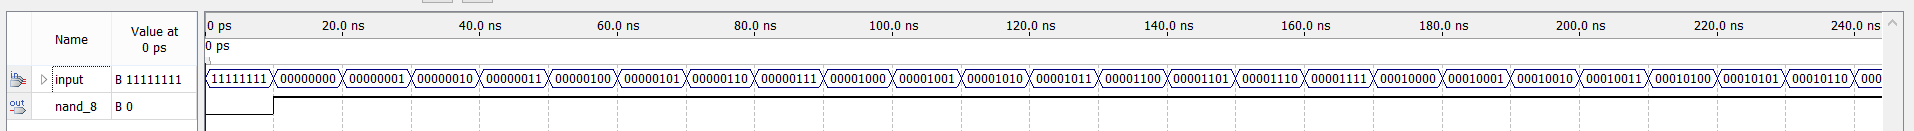
\includegraphics[scale=0.45]{pictures/Oevelse5/opg4/func_sim_8nand.JPG}
		\caption{Functional simulation af 8 input NAND gate}
		\label{fig:8innand}
	\end{figure}
\end{enumerate}
\clearpage





\newpage
\chapter{Øvelse 4}
\section{Opgave 1 - Binary circular watch}
\begin{enumerate}
	\item[1)]
	Vi skriver koden for vores cirkulære ur som det ses i kode \ref{lst:Watch}.\\
	\begin{lstlisting}[caption={VHDL code for binary circular watch},label={lst:Watch}]
	library ieee;
	use ieee.std_logic_1164.all;
	use ieee.numeric_std.all;
	
	entity watch is
	port( clk, speed, reset : in std_logic;
	mode : in std_logic_vector(1 downto 0);
	seg1 : out std_logic_vector(6 downto 0);
	cout : out std_logic);
	bin_val : out std_logic_vector(3 downto 0));
	end watch;
	
	architecture clock of watch is
	
	begin
	u2: entity work.counter port map(clk => clk_out, reset => reset, mode => mode, seg => seg1, cout => cout, bin_val => bin_val);
	
	
	process (reset, clk)
	variable clk_count : integer range 0 to 50000000;
	begin
	if reset = '0' then
	clk_count := 0;
	cout <= '0';
	elsif rising_edge(clk) then
	clk_count := clk_count + 1;
	cout <= '0';
	if speed = '1' then
	if clk_count >= 50000000 then
	cout <= '1';
	clk_count := 0;
	end if;
	elsif speed = '0' then
	if clk_count >= 25000 then
	cout <= '1';
	clk_count := 0;
	end if;
	end if;
	end if;
	
	end process;
	
	end clock;
	
	\end{lstlisting}
	
	Koden for vores counter er illustreret i kode \ref{lst:Counter}
	
		\begin{lstlisting}[caption={VHDL code for binary circular counter},label={lst:Counter}]
		library ieee;
		use ieee.std_logic_1164.all;
		use ieee.numeric_std.all;
		
		entity counter is
		port( clk, reset : in std_logic;
		mode : in std_logic_vector(1 downto 0);
		bin_val : out std_logic_vector(3 downto 0);
		cout : out std_logic;
		seg : out std_logic_vector(6 downto 0));	
		end counter;
		
		architecture circular of counter is
		signal bin_val_sig : std_logic_vector(3 downto 0);
		signal cout_sig : std_logic;
		begin
		
		u1: entity work.BCDdecoder port map(dcba => bin_val_sig, seg => seg);
		
		process (clk, reset, mode, bin_val_sig)
		
		begin
		if reset = '0' then
		bin_val_sig <= "0000";
		cout_sig <= '0';
		elsif rising_edge(clk) then
		if mode = "00" then
		if bin_val_sig = "1001" then 
		bin_val_sig <= "0000";
		cout_sig <= '1';
		else
		bin_val_sig <= std_logic_vector(unsigned(bin_val_sig)+1);
		cout_sig <= '0';
		end if;
		elsif mode = "01" then
		if bin_val_sig = "0101" then 
		bin_val_sig <= "0000";
		cout_sig <= '1';
		else
		bin_val_sig <= std_logic_vector(unsigned(bin_val_sig)+1);
		cout_sig <= '0';
		end if;
		else 
		if bin_val_sig = "0010" then 
		bin_val_sig <= "0000";
		cout_sig <= '1';
		else
		bin_val_sig <= std_logic_vector(unsigned(bin_val_sig)+1);
		cout_sig <= '0';
		end if;
		end if;
		
		end if;
		
		end process;
		bin_val <= bin_val_sig;
		cout <= cout_sig;
		end circular;
		
		\end{lstlisting}
		
		Vi har her anvendt endnu en VHDL-fil kaldet BCD-decoder, som vi i tidligere øvelser har anvendt til at decode vores værdier til visning på et 7-segment display.
		
		Da uret skal kunne tælle op for hvert 5. milisekund i speed-mode, skal counteren kun nå til 25000, som det ses i linje 34.
		
\item[2)] Vi tester vores watch på DE2-boardet. På følgende billeder kan forskellige værdier for 7-segment displayet 'hex0' ses:
		\begin{figure}[h]
			\centering
			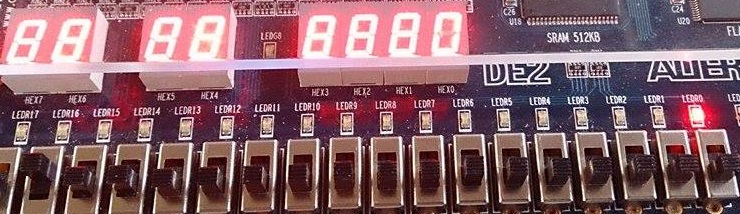
\includegraphics[scale=0.8]{pictures/Oevelse6/opg1/watch0.JPG}
			\caption{Uret er resat}
			\label{fig:alarm0}
		\end{figure}
		
		\begin{figure}[h]
			\centering
			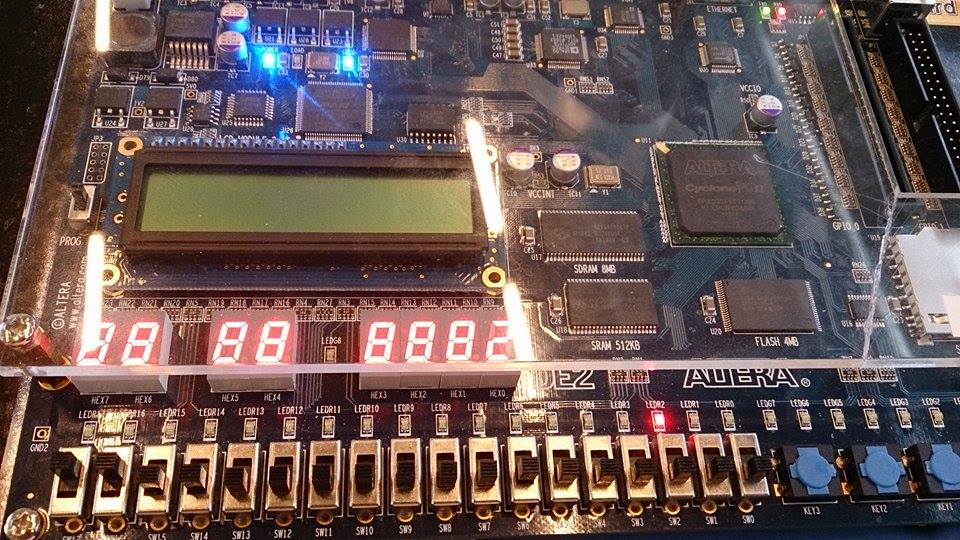
\includegraphics[scale=0.8]{pictures/Oevelse6/opg1/watch2.JPG}
			\caption{Uret viser 2}
			\label{fig:alarm2}
		\end{figure}

		\begin{figure}[h]
			\centering
			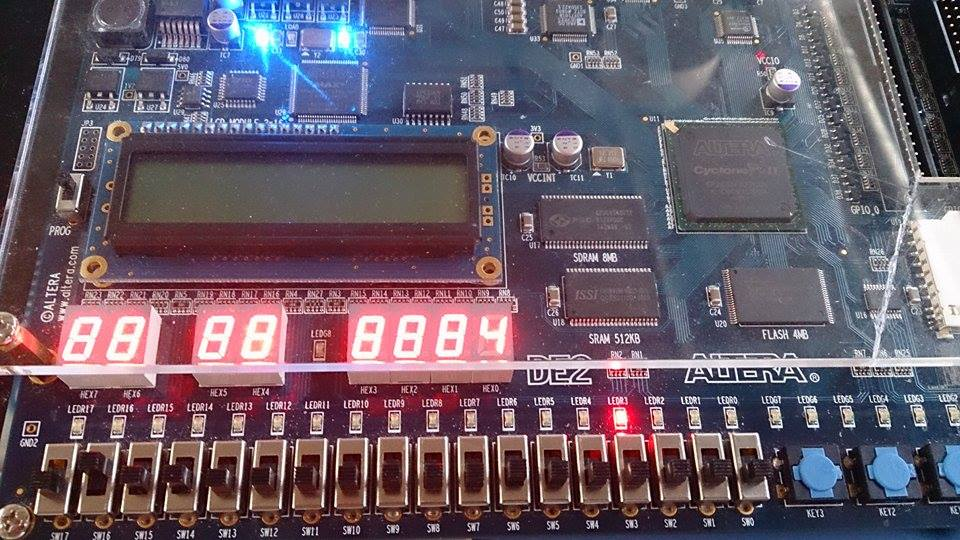
\includegraphics[scale=0.8]{pictures/Oevelse6/opg1/watch4.JPG}
			\caption{Uret viser 4}
			\label{fig:alarm4}
		\end{figure}


\end{enumerate}

\section{Opgave 2 - Full-adder}
	\flushleft
\begin{enumerate}
	\item[1)]
	Med to half-addere kan man lave en full-adder. Dette vil vi nu implementere i hhv. dataflow-style, behavioral-style og structural-style.\\
	\medskip
	\begin{lstlisting}[caption={Full-adder Dataflow VHDL kode},label={lst:FaDataflowCode}]
	library ieee;
	use ieee.std_logic_1164.all;
	
	entity full_adder_dataflow is
	port (a, b, carry_in : in std_logic;
	sum, carry_out : out std_logic);
	end full_adder_dataflow;
	
	architecture dataflow of full_adder_dataflow is
	
	signal s1, s2, s3 : std_logic;
	begin
	s1 <= a xor b; 
	sum <= s1 xor carry_in;
	s2 <= s1 and carry_in;
	s3 <= a and b;
	carry_out <= s2 or s3;
	
	end dataflow;
	\end{lstlisting}
	\medskip
	\begin{lstlisting}[caption={Full-adder Behavioral VHDL kode}, label={lst:FaBehavioralCode}]
	library ieee;
	use ieee.std_logic_1164.all;
	
	entity full_adder_behavioral is
	port (a, b, carry_in : in std_logic;
	sum, carry_out : out std_logic);
	end full_adder_behavioral;
	
	architecture behavioral of full_adder_behavioral is
	
	signal s1, s2, s3 : std_logic;
	begin
	fa: process (carry_in, a, b)
	begin
	if carry_in = '0'  then
	
	if a = '1' then
	sum <= not b;
	carry_out <= b;
	else
	sum <= b;
	carry_out <= '0';
	end if;
	else 
	sum <= a xnor b;
	carry_out <= a or b;
	end if;
	end process fa;
	
	end behavioral;
	\end{lstlisting}
	\medskip
	\begin{lstlisting}[caption={Full-adder Structural VHDL kode},label={lst:FaStructuralCode}]
	library ieee;
	use ieee.std_logic_1164.all;
	
	entity full_adder_structural is
	port (a, b, carry_in : in std_logic;
	sum, carry_out : out std_logic);
	end full_adder_structural;
	
	architecture structural of full_adder_structural is
	
	signal s1, s2, s3 : std_logic;
	begin
	
	ha1: entity work.half_adder_dataflow port map (a => a, b => b, sum => s1, carry_out => s3);
	ha2: entity work.half_adder_dataflow port map (a => s1, b => carry_in, sum => sum, carry_out => s2);
	or1: entity work.or_2 port map (i1 => s2, i2 => s3, o1 => carry_out);
	
	end structural;
	\end{lstlisting}
	\newpage
	\flushleft
		\item[2)]
		Med et RTL view kan vi se hvordan de tre forskellige koder vil blive omdannet til logiske gates.\\
		\begin{figure}[h]
		\centering
		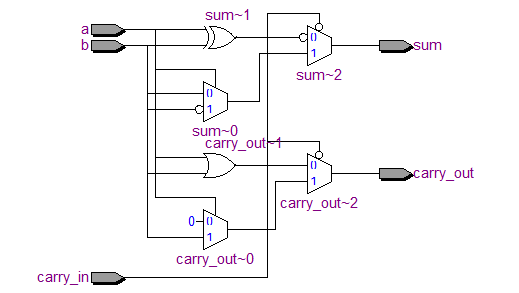
\includegraphics[scale=0.7]{pictures/Oevelse1/Full_adder/Behavioral_RTL.JPG}
		\caption{Full-adder - Behavioral RTL view}
		\label{fig:FaBehavioralRTL}
	\end{figure}
	
	\begin{figure}[h]
		\centering
		\includegraphics[scale=0.7]{pictures/Oevelse1/Full_adder/dataflow_RTL.JPG}
		\caption{Full-adder - Dataflow RTL view}
		\label{fig:FaDataflowRTL}	
	\end{figure}
	
	\begin{figure}[h]
		\centering
		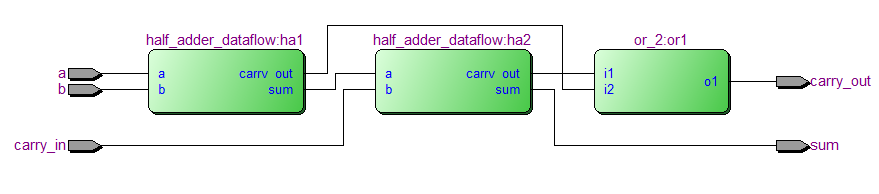
\includegraphics[scale=0.7]{pictures/Oevelse1/Full_adder/Structural_RTL.JPG}
		\caption{Full-adder - Structural RTL view}
		\label{fig:FaStructuralRTL}	
	\end{figure}
	
	\newpage
	\flushleft
		\item[3)]
		Til sidst laver vi en functional simulering for at se om vores tre full-adder koder opfører sig som vi ønsker.\\	

	\begin{figure}[h]
		\centering
		\includegraphics[scale=0.8]{pictures/Oevelse1/Full_adder/Dataflow_functional_simulation.jpg}
		\caption{Full-adder - Dataflow functional Simulation}
		\label{fig:FaDataflowFunctionalSim}
	\end{figure}
	\begin{figure}[h]
		\centering
		\includegraphics[scale=0.8]{pictures/Oevelse1/Full_adder/Behavioral_functional_simulation.jpg}
		\caption{Full-adder - Behavioral functional Simulation}
		\label{fig:FaBehavioralFunctionalSim}
	\end{figure}
	\begin{figure}[h]
		\centering
		\includegraphics[scale=0.6]{pictures/Oevelse1/Full_adder/Structural_functional_simulation.jpg}
		\caption{Full-adder - Structural functional Simulation}
		\label{fig:FaStructuralFunctionalSim}
	\end{figure}
	\newpage

\end{enumerate}


\section{Opgave 3 - Guess a HEX number game}
\begin{enumerate}
	\item[1)]
	Vi skriver koden for vores Guessgame som det ses på figur \ref{lst:Guessgame}.\\
	\begin{lstlisting}[caption={Behavioral style kode for Guessgame},label={lst:Guessgame}]
library ieee;
use ieee.std_logic_1164.all;
use ieee.numeric_std.all;

entity guessgame is 
port (input : in std_logic_vector(7 downto 0);
set, show, try : in std_logic;
seg1, seg10 : out std_logic_vector(6 downto 0));
end guessgame;

architecture game_process of guessgame is
signal i_input10 : std_logic_vector(7 downto 4);
signal i_input1 : std_logic_vector(3 downto 0);
signal i_seg1, i_seg10 : std_logic_vector(3 downto 0);
begin
count: process (set, show, try)

variable target : std_logic_vector(7 downto 0);

begin

--target := "00000000";

if set = '0' then target := input;
elsif show = '0' then 
i_seg1 <= target(3 downto 0);
i_seg10 <= target(7 downto 4);
case i_seg1 is
when "0000" => seg1 <= "0000001"; -- 0
when "0001" => seg1 <= "1001111"; -- 1
when "0010" => seg1 <= "0010010"; -- 2
when "0011" => seg1 <= "0000110"; -- 3
when "0100" => seg1 <= "1001100"; -- 4
when "0101" => seg1 <= "0100100"; -- 5
when "0110" => seg1 <= "0100000"; -- 6
when "0111" => seg1 <= "0001111"; -- 7
when "1000" => seg1 <= "0000000"; -- 8
when "1001" => seg1 <= "0001100"; -- 9
when "1010" => seg1 <= "0001000"; -- A
when "1011" => seg1 <= "1100000"; -- B
when "1100" => seg1 <= "0110001"; -- C
when "1101" => seg1 <= "1000010"; -- D
when "1110" => seg1 <= "0110000"; -- E
when "1111" => seg1 <= "0111000"; -- F
when others => seg1 <= "1111111"; -- Slukket
end case;
case i_seg10 is
when "0000" => seg10 <= "0000001"; -- 0
when "0001" => seg10 <= "1001111"; -- 1
when "0010" => seg10 <= "0010010"; -- 2
when "0011" => seg10 <= "0000110"; -- 3
when "0100" => seg10 <= "1001100"; -- 4
when "0101" => seg10 <= "0100100"; -- 5
when "0110" => seg10 <= "0100000"; -- 6
when "0111" => seg10 <= "0001111"; -- 7
when "1000" => seg10	<= "0000000"; -- 8
when "1001" => seg10	<= "0001100"; -- 9
when "1010" => seg10 <= "0001000"; -- A
when "1011" => seg10 <= "1100000"; -- B
when "1100" => seg10 <= "0110001"; -- C
when "1101" => seg10	<= "1000010"; -- D
when "1110" => seg10 <= "0110000"; -- E
when "1111" => seg10 <= "0111000"; -- F
when others => seg10 <= "1111111"; -- Slukket
end case;
elsif try = '0' then 
if input > target then --output Hi
seg10 <= "1001000"; 
seg1 <= "1111001";
elsif input < target then -- output Lo
seg10 <= "1110001"; 
seg1 <= "1100010";
elsif input = target then -- output --
seg10 <= "1111110"; 
seg1 <= "1111110";
end if;
elsif set = '1' and show = '1' and try = '1' then 
i_input10 <= input(7 downto 4); 
i_input1 <= input(3 downto 0);
case i_input1 is
when "0000" => seg1 <= "0000001"; -- 0
when "0001" => seg1 <= "1001111"; -- 1
when "0010" => seg1 <= "0010010"; -- 2
when "0011" => seg1 <= "0000110"; -- 3
when "0100" => seg1 <= "1001100"; -- 4
when "0101" => seg1 <= "0100100"; -- 5
when "0110" => seg1 <= "0100000"; -- 6
when "0111" => seg1 <= "0001111"; -- 7
when "1000" => seg1 <= "0000000"; -- 8
when "1001" => seg1 <= "0001100"; -- 9
when "1010" => seg1 <= "0001000"; -- A
when "1011" => seg1 <= "1100000"; -- B
when "1100" => seg1 <= "0110001"; -- C
when "1101" => seg1 <= "1000010"; -- D
when "1110" => seg1 <= "0110000"; -- E
when "1111" => seg1 <= "0111000"; -- F
when others => seg1 <= "1111111"; -- Slukket
end case;

case i_input10 is
when "0000" => seg10 <= "0000001"; -- 0
when "0001" => seg10 <= "1001111"; -- 1
when "0010" => seg10 <= "0010010"; -- 2
when "0011" => seg10 <= "0000110"; -- 3
when "0100" => seg10 <= "1001100"; -- 4
when "0101" => seg10 <= "0100100"; -- 5
when "0110" => seg10 <= "0100000"; -- 6
when "0111" => seg10 <= "0001111"; -- 7
when "1000" => seg10 <= "0000000"; -- 8
when "1001" => seg10 <= "0001100"; -- 9
when "1010" => seg10 <= "0001000"; -- A
when "1011" => seg10 <= "1100000"; -- B
when "1100" => seg10 <= "0110001"; -- C
when "1101" => seg10 <= "1000010"; -- D
when "1110" => seg10 <= "0110000"; -- E
when "1111" => seg10 <= "0111000"; -- F
when others => seg10 <= "1111111"; -- Slukket
end case;
end if;
end process count;
end game_process;


	\end{lstlisting}
	\item[2)]
	Vi downloader programmet til vores DE2-board, hvor SW[0-3] vises på HEX0, SW[4-7] vises på HEX1, KEY3 = set, KEY2 = show og KEY1 = try. \\
	\begin{figure}[h]
		\centering
		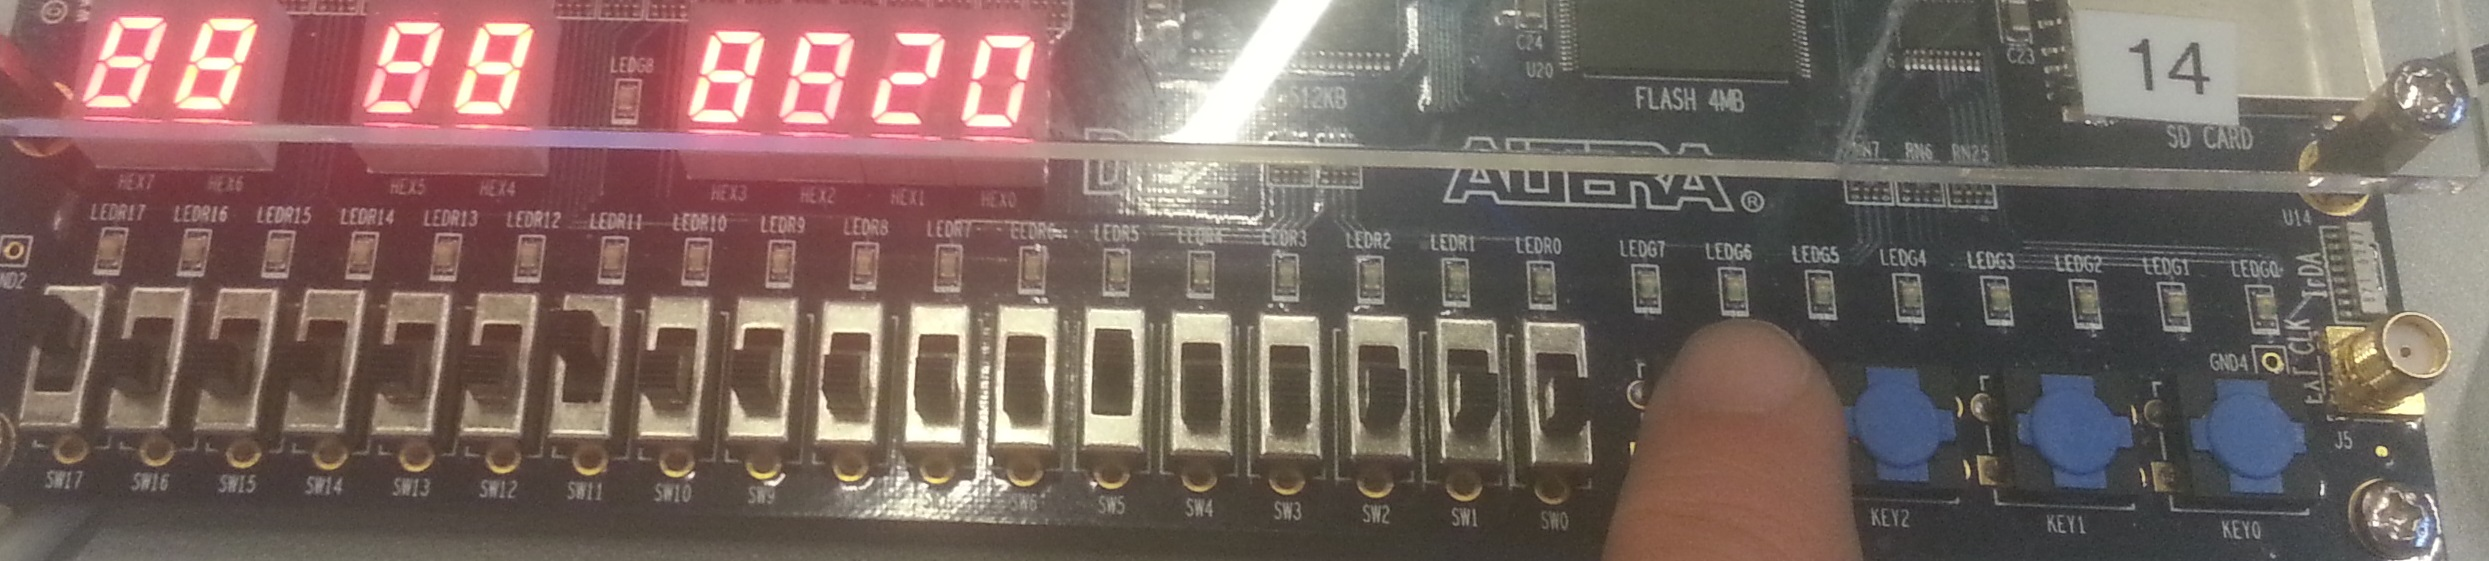
\includegraphics[scale=0.8]{pictures/Oevelse5/opg3/guess_set.JPG}
		\caption{}
		\label{fig:GuessSet}
	\end{figure}
	\begin{figure}[h]
		\centering
		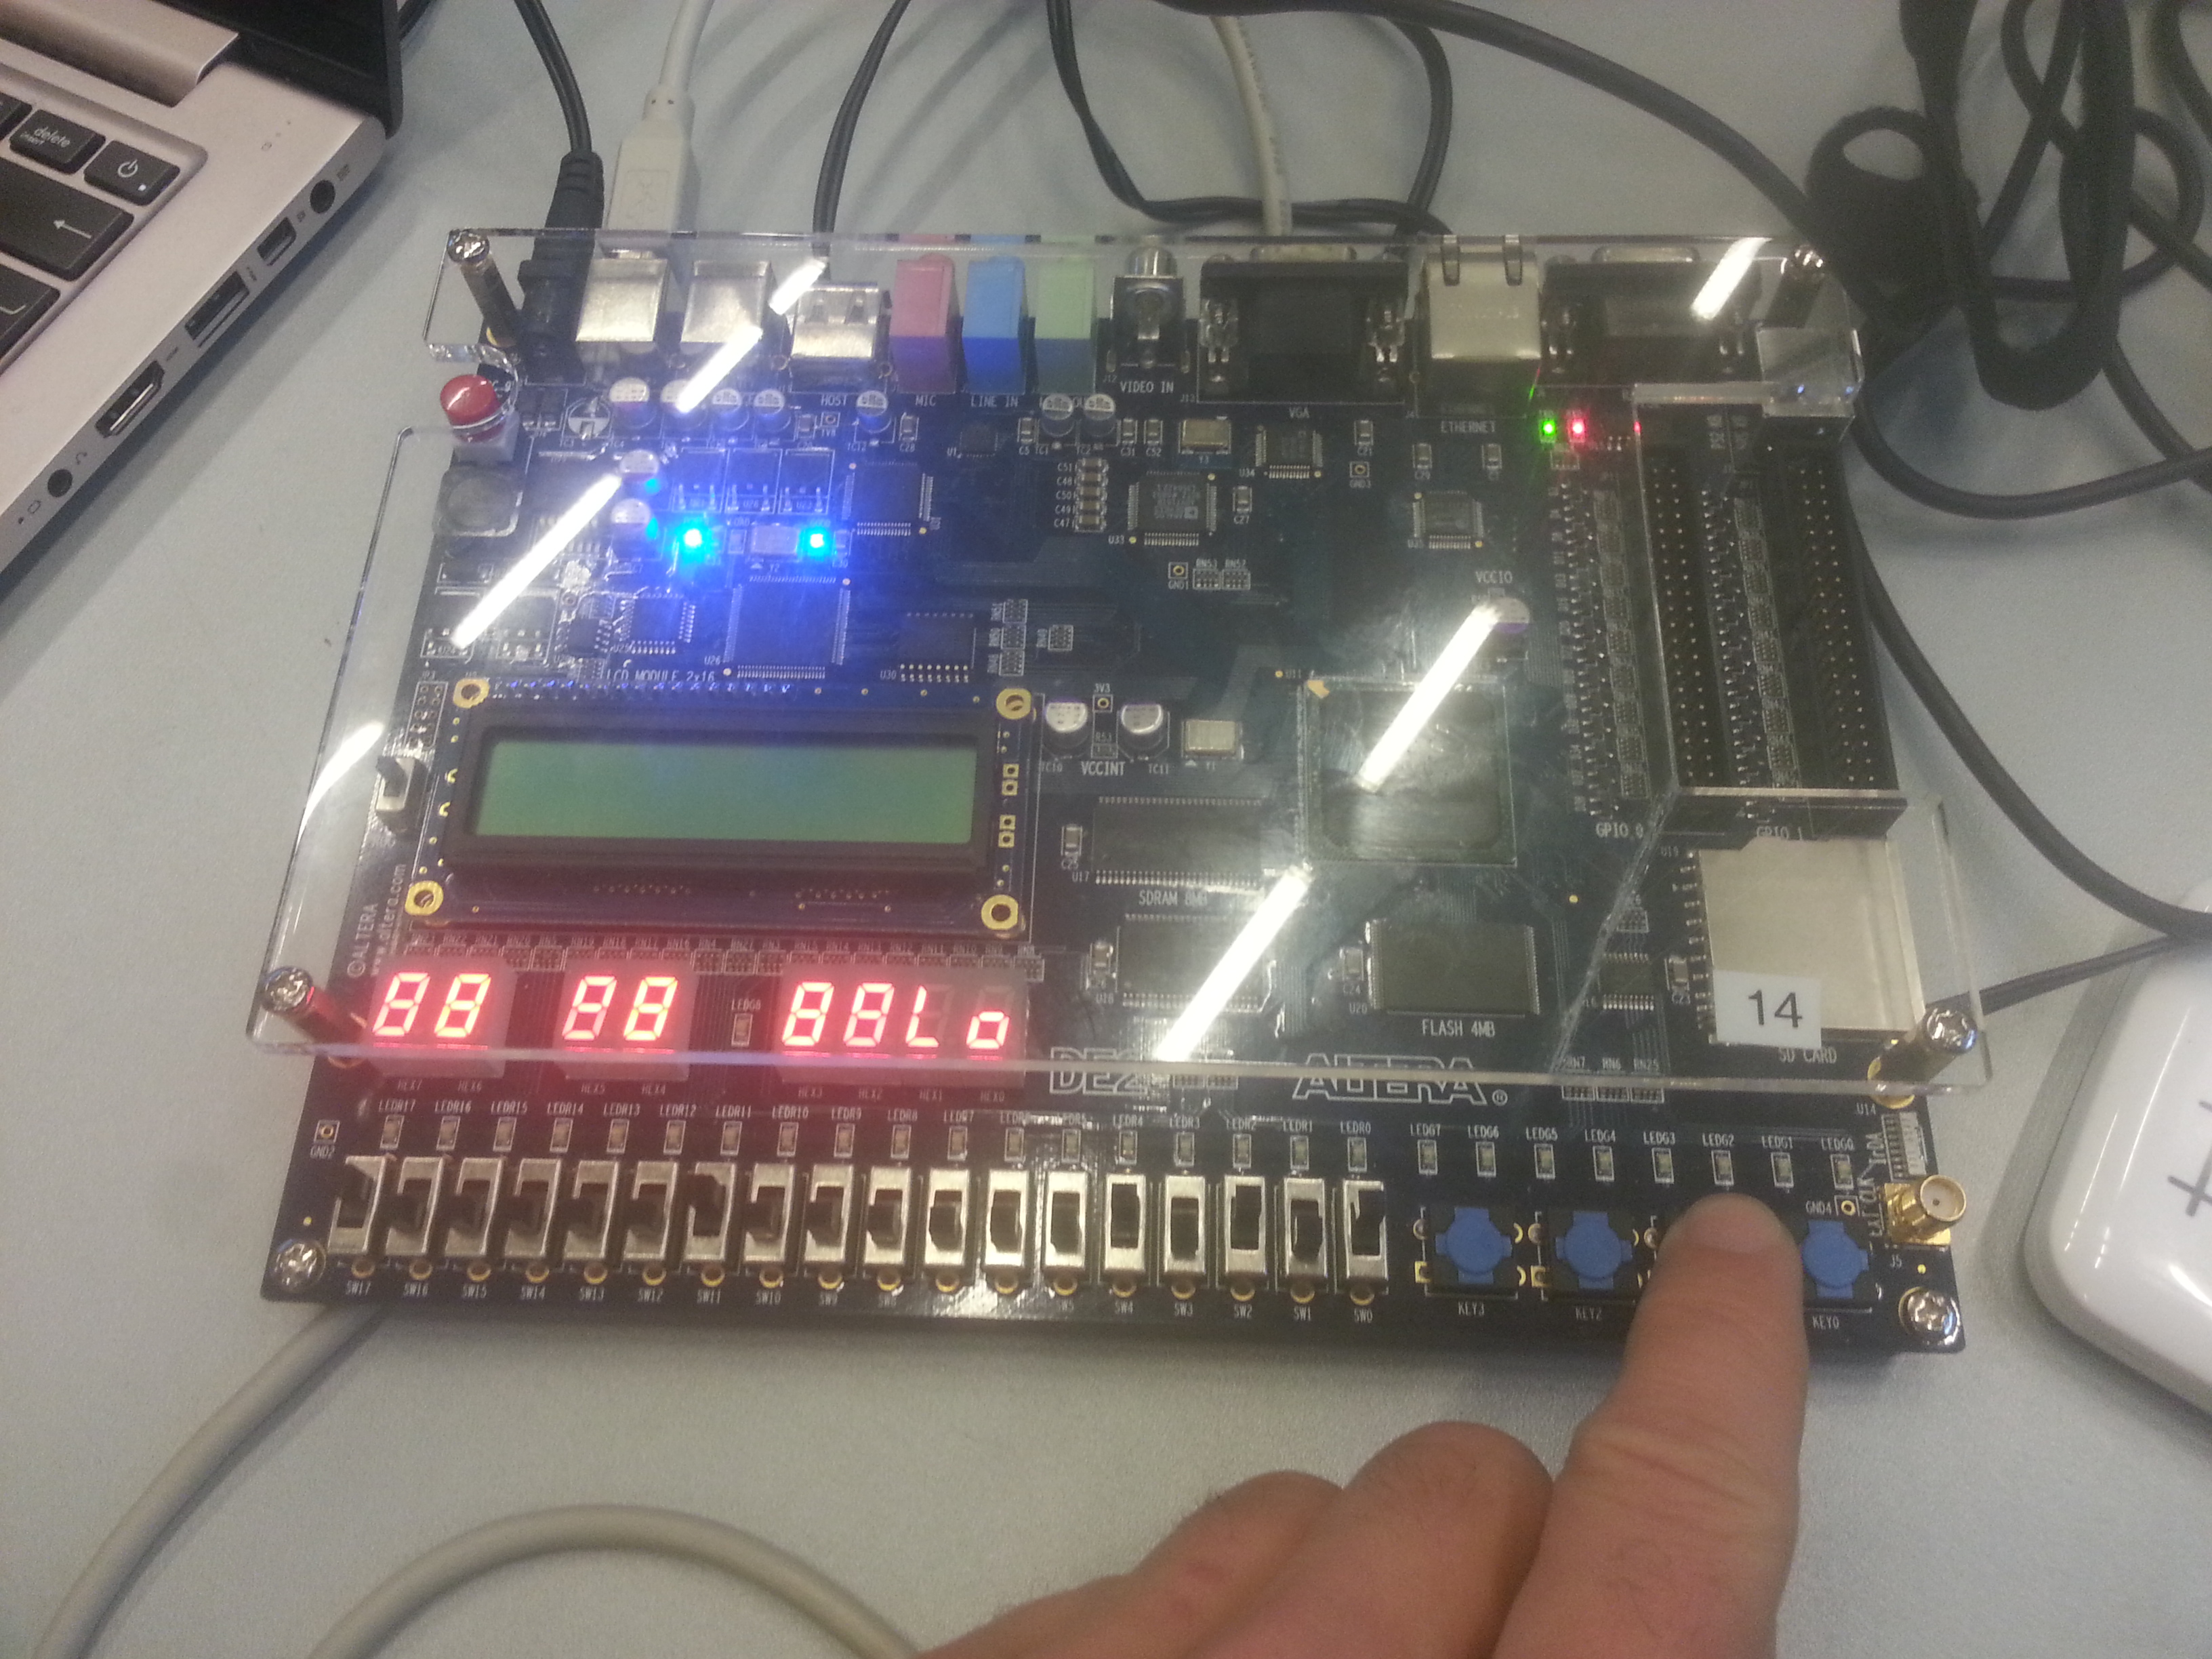
\includegraphics[scale=0.8]{pictures/Oevelse5/opg3/guess_try_lo.JPG}
		\caption{}
		\label{fig:GuessTryLo}
	\end{figure}
	\begin{figure}[h]
		\centering
		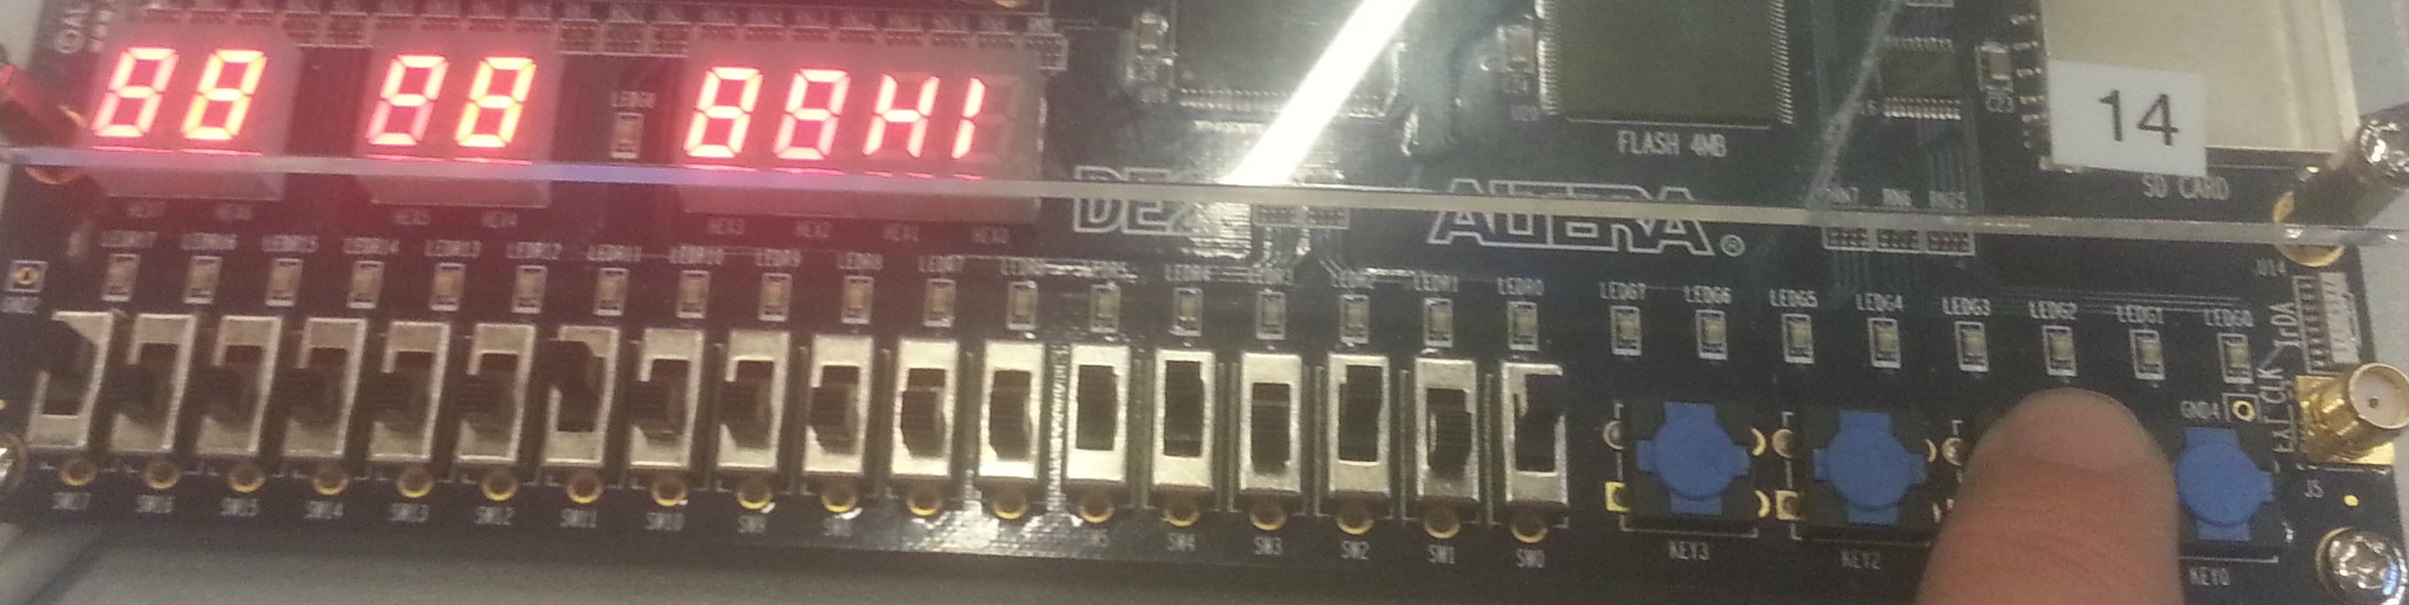
\includegraphics[scale=0.8]{pictures/Oevelse5/opg3/guess_try_hi.JPG}
		\caption{}
		\label{fig:GuessTryHi}
	\end{figure}
	\begin{figure}[h]
		\centering
		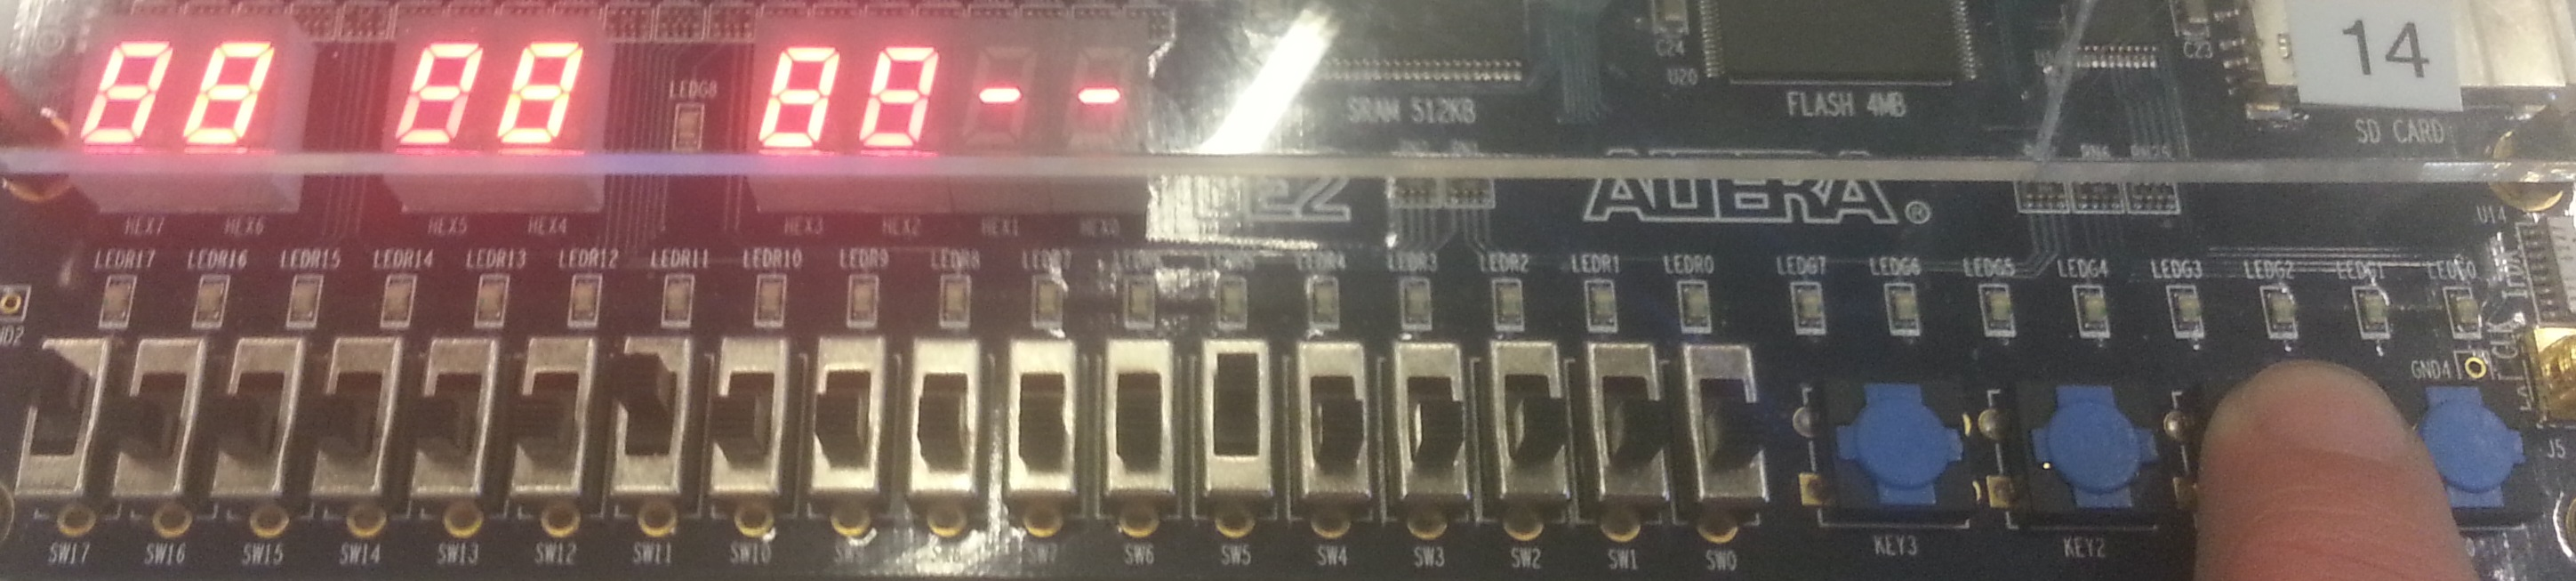
\includegraphics[scale=0.8]{pictures/Oevelse5/opg3/guess_try_ok.JPG}
		\caption{}
		\label{fig:GuessTryOk}
	\end{figure}
	\begin{figure}[h]
		\centering
		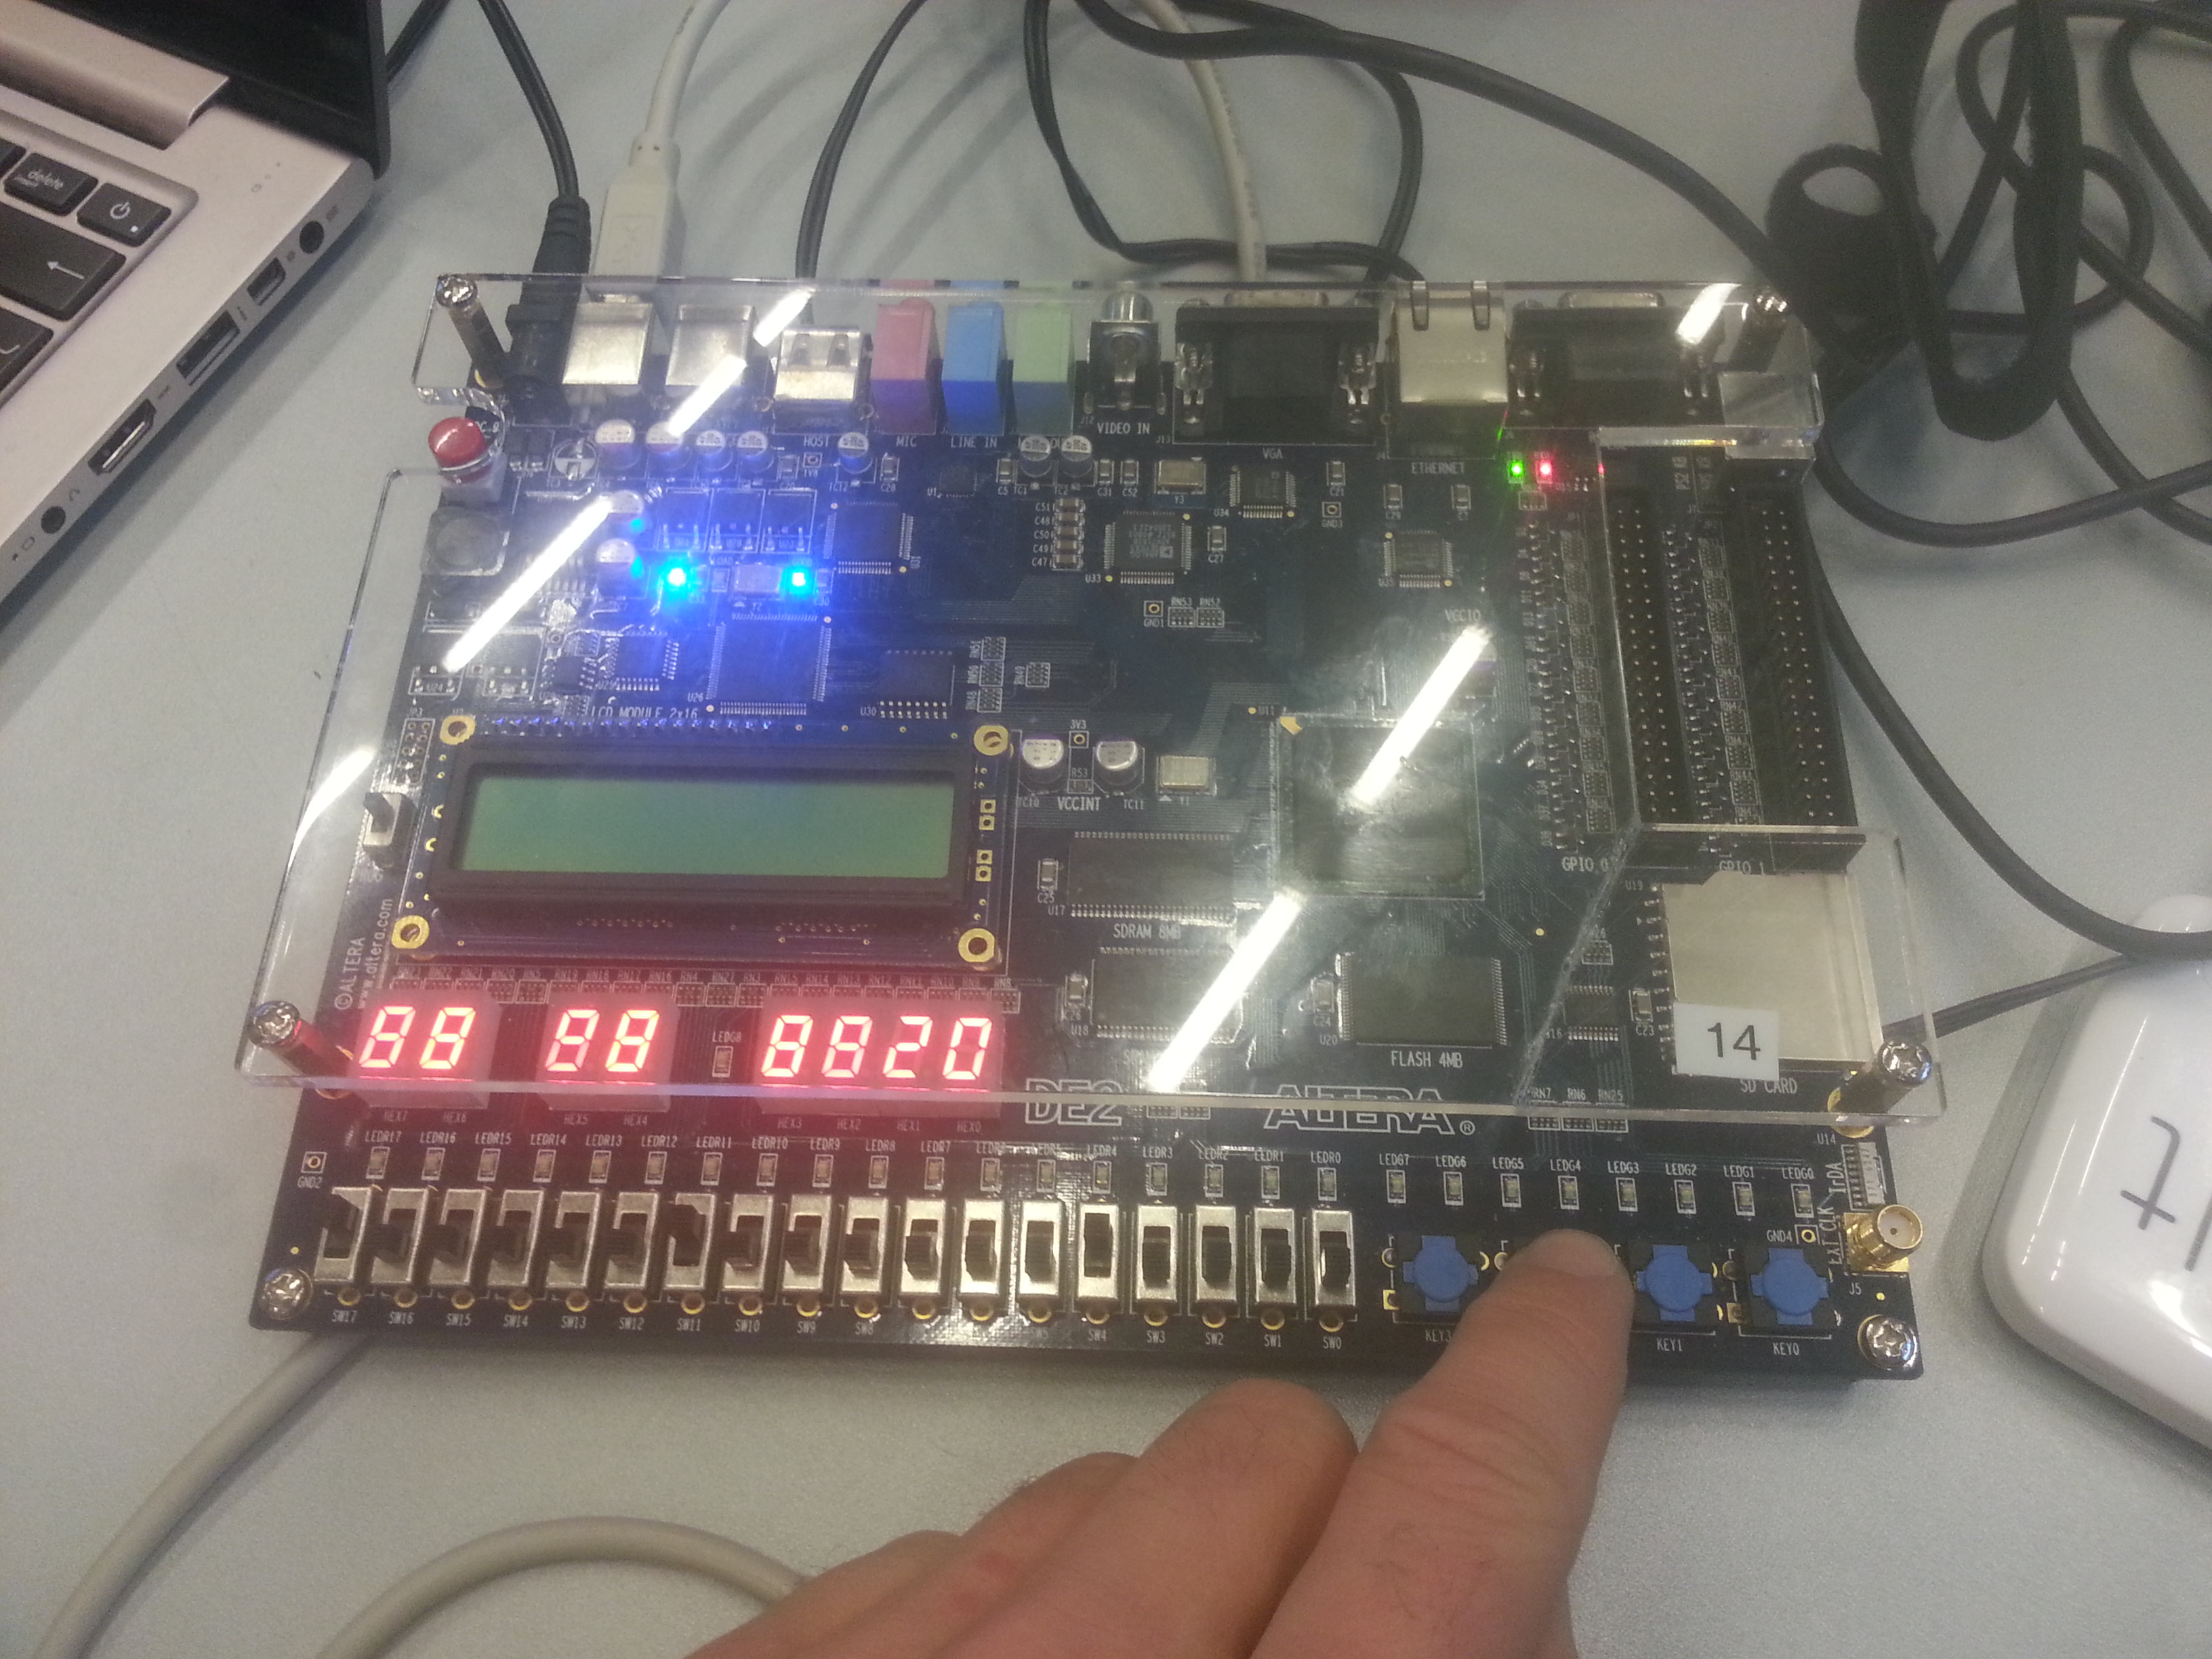
\includegraphics[scale=0.8]{pictures/Oevelse5/opg3/guess_show.JPG}
		\caption{}
		\label{fig:GuessShow}
	\end{figure}
		\item[1)]
		Vi skriver koden for vores Guessgame som det ses på figur \ref{lst:Guessgame}.\\
		\begin{lstlisting}[caption={Behavioral style kode for Guessgame},label={lst:Guessgame}]
		library ieee;
		use ieee.std_logic_1164.all;
		use ieee.numeric_std.all;
		
		entity guessgame is 
		port (input : in std_logic_vector(7 downto 0);
		set, show, try : in std_logic;
		seg1, seg10 : out std_logic_vector(6 downto 0));
		end guessgame;
		
		architecture game_process of guessgame is
		signal i_input10 : std_logic_vector(7 downto 4);
		signal i_input1 : std_logic_vector(3 downto 0);
		signal i_seg1, i_seg10 : std_logic_vector(3 downto 0);
		begin
		count: process (set, show, try)
		
		variable target : std_logic_vector(7 downto 0);
		
		begin
		
		--target := "00000000";
		
		if set = '0' then target := input;
		elsif show = '0' then 
		i_seg1 <= target(3 downto 0);
		i_seg10 <= target(7 downto 4);
		case i_seg1 is
		when "0000" => seg1 <= "0000001"; -- 0
		when "0001" => seg1 <= "1001111"; -- 1
		when "0010" => seg1 <= "0010010"; -- 2
		when "0011" => seg1 <= "0000110"; -- 3
		when "0100" => seg1 <= "1001100"; -- 4
		when "0101" => seg1 <= "0100100"; -- 5
		when "0110" => seg1 <= "0100000"; -- 6
		when "0111" => seg1 <= "0001111"; -- 7
		when "1000" => seg1 <= "0000000"; -- 8
		when "1001" => seg1 <= "0001100"; -- 9
		when "1010" => seg1 <= "0001000"; -- A
		when "1011" => seg1 <= "1100000"; -- B
		when "1100" => seg1 <= "0110001"; -- C
		when "1101" => seg1 <= "1000010"; -- D
		when "1110" => seg1 <= "0110000"; -- E
		when "1111" => seg1 <= "0111000"; -- F
		when others => seg1 <= "1111111"; -- Slukket
		end case;
		case i_seg10 is
		when "0000" => seg10 <= "0000001"; -- 0
		when "0001" => seg10 <= "1001111"; -- 1
		when "0010" => seg10 <= "0010010"; -- 2
		when "0011" => seg10 <= "0000110"; -- 3
		when "0100" => seg10 <= "1001100"; -- 4
		when "0101" => seg10 <= "0100100"; -- 5
		when "0110" => seg10 <= "0100000"; -- 6
		when "0111" => seg10 <= "0001111"; -- 7
		when "1000" => seg10	<= "0000000"; -- 8
		when "1001" => seg10	<= "0001100"; -- 9
		when "1010" => seg10 <= "0001000"; -- A
		when "1011" => seg10 <= "1100000"; -- B
		when "1100" => seg10 <= "0110001"; -- C
		when "1101" => seg10	<= "1000010"; -- D
		when "1110" => seg10 <= "0110000"; -- E
		when "1111" => seg10 <= "0111000"; -- F
		when others => seg10 <= "1111111"; -- Slukket
		end case;
		elsif try = '0' then 
		if input > target then --output Hi
		seg10 <= "1001000"; 
		seg1 <= "1111001";
		elsif input < target then -- output Lo
		seg10 <= "1110001"; 
		seg1 <= "1100010";
		elsif input = target then -- output --
		seg10 <= "1111110"; 
		seg1 <= "1111110";
		end if;
		elsif set = '1' and show = '1' and try = '1' then 
		i_input10 <= input(7 downto 4); 
		i_input1 <= input(3 downto 0);
		case i_input1 is
		when "0000" => seg1 <= "0000001"; -- 0
		when "0001" => seg1 <= "1001111"; -- 1
		when "0010" => seg1 <= "0010010"; -- 2
		when "0011" => seg1 <= "0000110"; -- 3
		when "0100" => seg1 <= "1001100"; -- 4
		when "0101" => seg1 <= "0100100"; -- 5
		when "0110" => seg1 <= "0100000"; -- 6
		when "0111" => seg1 <= "0001111"; -- 7
		when "1000" => seg1 <= "0000000"; -- 8
		when "1001" => seg1 <= "0001100"; -- 9
		when "1010" => seg1 <= "0001000"; -- A
		when "1011" => seg1 <= "1100000"; -- B
		when "1100" => seg1 <= "0110001"; -- C
		when "1101" => seg1 <= "1000010"; -- D
		when "1110" => seg1 <= "0110000"; -- E
		when "1111" => seg1 <= "0111000"; -- F
		when others => seg1 <= "1111111"; -- Slukket
		end case;
		
		case i_input10 is
		when "0000" => seg10 <= "0000001"; -- 0
		when "0001" => seg10 <= "1001111"; -- 1
		when "0010" => seg10 <= "0010010"; -- 2
		when "0011" => seg10 <= "0000110"; -- 3
		when "0100" => seg10 <= "1001100"; -- 4
		when "0101" => seg10 <= "0100100"; -- 5
		when "0110" => seg10 <= "0100000"; -- 6
		when "0111" => seg10 <= "0001111"; -- 7
		when "1000" => seg10 <= "0000000"; -- 8
		when "1001" => seg10 <= "0001100"; -- 9
		when "1010" => seg10 <= "0001000"; -- A
		when "1011" => seg10 <= "1100000"; -- B
		when "1100" => seg10 <= "0110001"; -- C
		when "1101" => seg10 <= "1000010"; -- D
		when "1110" => seg10 <= "0110000"; -- E
		when "1111" => seg10 <= "0111000"; -- F
		when others => seg10 <= "1111111"; -- Slukket
		end case;
		end if;
		end process count;
		end game_process;
		
		
		\end{lstlisting}
		\item[2)]
		Vi downloader programmet til vores DE2-board, hvor SW[0-3] vises på HEX0, SW[4-7] vises på HEX1, KEY3 = set, KEY2 = show og KEY1 = try. \\
		\begin{figure}[h]
			\centering
			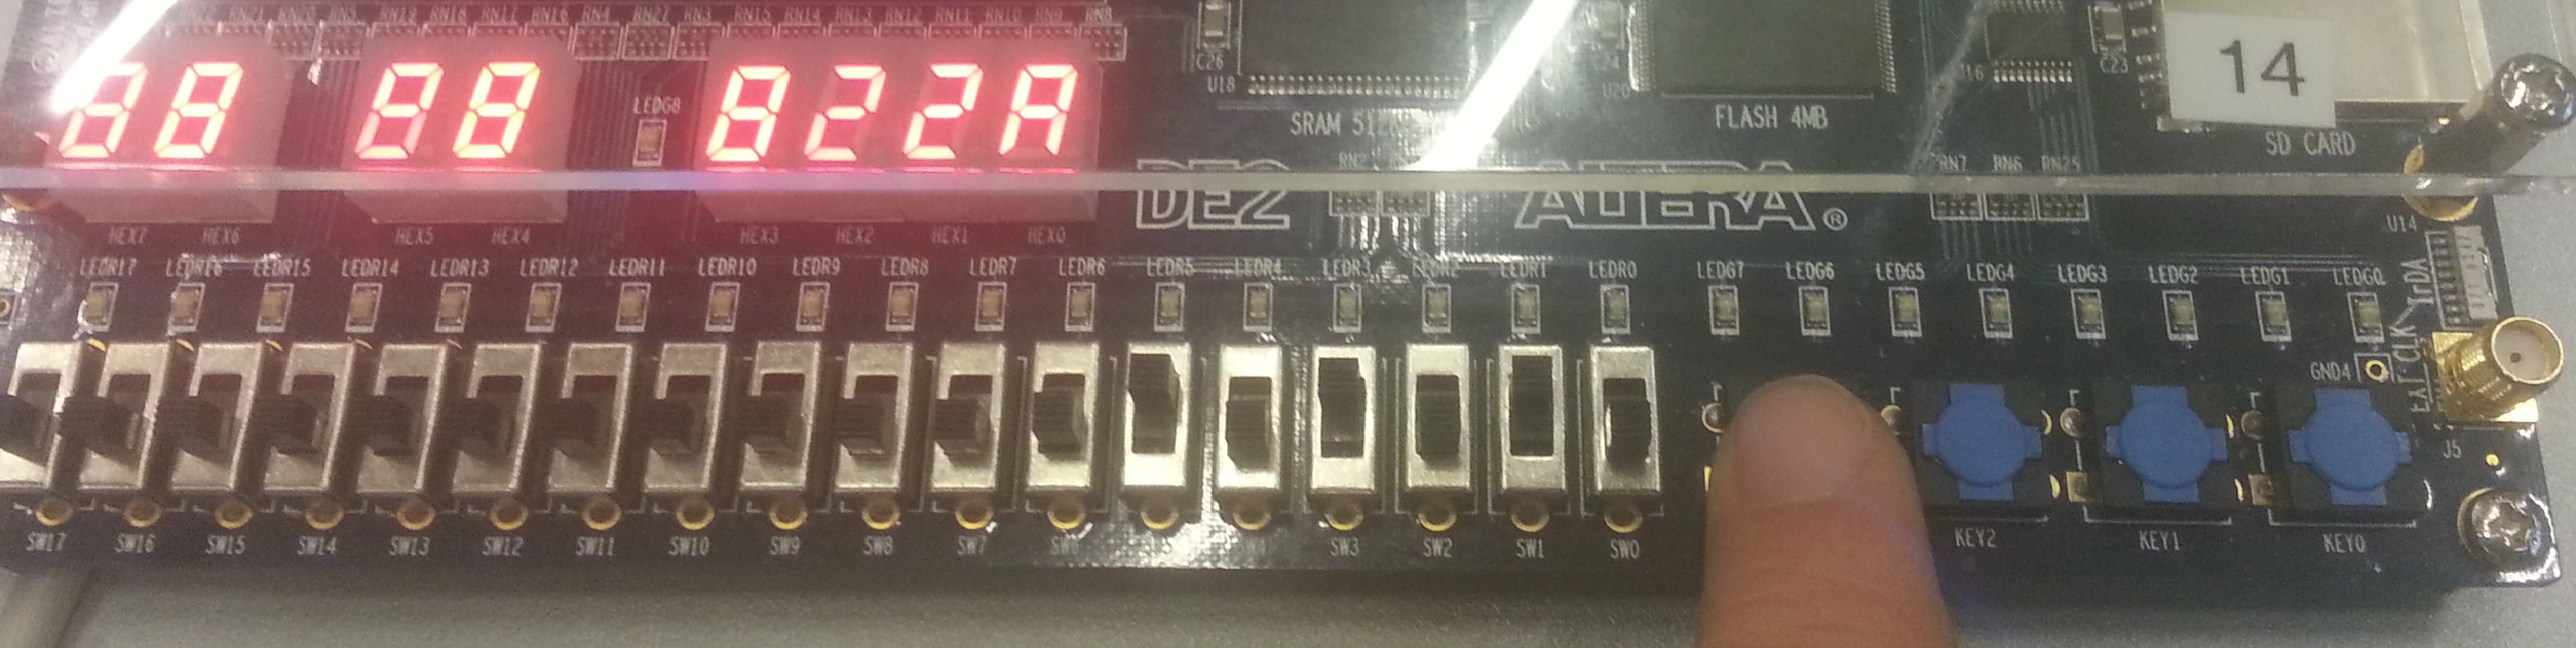
\includegraphics[scale=0.15]{pictures/Oevelse5/opg3/guess_2p_set.JPG}
			\caption{Tal sættes af player 2}
			\label{fig:Guess2pSet}
		\end{figure}
		\begin{figure}[h]
			\centering
			\includegraphics[scale=0.15]{pictures/Oevelse5/opg3/guess_2p_try_lo.JPG}
			\caption{Tal gættes af player 1 og findes for lavt}
			\label{fig:Guess2pTryLo}
		\end{figure}
		\begin{figure}[h]
			\centering
			\includegraphics[scale=0.15]{pictures/Oevelse5/opg3/guess_2p_try_hi.JPG}
			\caption{Tal gættes af player 1 og findes for højt}
			\label{fig:Guess2pTryHi}
		\end{figure}
		\begin{figure}[h]
			\centering
			\includegraphics[scale=0.15]{pictures/Oevelse5/opg3/guess_2p_try_ok.JPG}
			\caption{Tal gættes af player 2 og er korrekt}
			\label{fig:Guess2pTryOk}
		\end{figure}
		\begin{figure}[h]
			\centering
			\includegraphics[scale=0.15]{pictures/Oevelse5/opg3/guess_2p_show.JPG}
			\caption{Player 1 viser gemte tal}
			\label{fig:Guess2pShow}
		\end{figure}
\end{enumerate}
\section{Opgave 4 - 8 input NAND using the for loop}
\begin{enumerate}
	\item[1)]
	Vi skriver koden for en 8 input NAND gate ved hjælp af en for løkke i behavioral style som det ses på figur \ref{lst:8innand}.\\
	\begin{lstlisting}[caption={Behavioral style kode for en 8 input NAND gate},label={lst:8innand}]
	library ieee;
	use ieee.std_logic_1164.all;
	
	entity inNAND is
	port (input : in std_logic_vector(7 downto 0);
	nand_8 : out std_logic);
	end inNAND;
	
	architecture nand_process of inNAND is
	begin
	comp: process (input)
	begin
	nand_8 <='0';
	
	for i in 7 downto 0 loop
	if (input(i) = '0') then nand_8 <= '1'; 
	exit;
	end if;
	end loop;
	end process comp;
	end nand_process;
	\end{lstlisting}
	Jævnfør linje 13: Forudsætter at alle input er høje, og dermed output = 0\\
	Jævnfør linje 16: Hvis bare ét input er lavt, vil output blive 1\\

	Med en functional simulation ser vi at koden virker efter hensigten, som det ses på figur \ref{fig:8innand}.\\
	\begin{figure}[h]
		\centering
		\includegraphics[scale=0.45]{pictures/Oevelse5/opg4/func_sim_8nand.JPG}
		\caption{Functional simulation af 8 input NAND gate}
		\label{fig:8innand}
	\end{figure}
\end{enumerate}
\clearpage





\end{document}
